\documentclass{article}
\usepackage[left=0.85in, right=0.85in, top=0.5in, bottom=0.95in]{geometry}
\usepackage[T1]{fontenc}
\usepackage[utf8]{inputenc}
\usepackage[italian]{babel}
\usepackage{pdfpages}
\usepackage{graphicx}
\usepackage{wrapfig2}
\usepackage{amsmath}
\usepackage{amsthm}
\usepackage{amssymb}
\usepackage{cases}
\usepackage{gensymb} %simboli come ° = \degree  etc etc
\usepackage{subcaption}
\usepackage{hyperref}
\hypersetup{
	colorlinks=true,
	linkcolor=blue,    
	urlcolor=blue,
	%pdfpagemode=FullScreen,
}
\urlstyle{same}
\usepackage{changepage}
\usepackage{lastpage, epstopdf}
\usepackage{fancyhdr}
\usepackage{tcolorbox}
%\usepackage{background}
\usepackage{tikz}
\usetikzlibrary{patterns}
\usetikzlibrary{mindmap}
\usepackage{pgfplots}


%=======HEADER & FOOTER=======%
\def\lesson{Lezione N. 13,14,15}
\def\outcome{\textbf{Learning Outcomes:} Outcomes go here. }

\pagestyle{fancy}
\fancyhf{}
\renewcommand{\headrulewidth}{0pt}
\renewcommand{\footrulewidth}{1.4pt}
\lfoot{A.M. $\diamond$ \the\year}
\cfoot{Page \thepage}
\rfoot{\lesson}

%=======CORNELL STYLE FORMAT=======%
%\SetBgScale{1}
%\SetBgAngle{0}
%\SetBgColor{black}
%\SetBgContents{\rule{1pt}{0.85\paperheight}}
%\SetBgHshift{-1.6in}
%\SetBgVshift{-0.1in}

%=======CUSTOM BOXES=======%

\parindent 0ex

%=======BODY=======%
\begin{document}
	\setcounterpageref{secnumdepth}{0}
	\section*{Parte 10} %Date: \hrulefill}
%	\begin{tcolorbox}{\outcome}\end{tcolorbox}

\begin{adjustwidth}{2in}{} 
	
\textbf{{\Large Fatica}} \mbox{} \newline
		Si sono visti finora dei semplici modelli analitici che interpretano il comportamento statico di componenti meccanici, questi  soggetti, nelle ipotesi di De Saint Venant, a carichi statici, costanti nel tempo; nella realtà un carico perfettamente constante nel tempo non esiste, è un'idealizzazione. 
		
		Solo nel caso in cui le variazioni di tensione sono piccole e il gradiente delle stesse è sufficientemente piccolo l'approssimazione con una sollecitazione statica diviene plausibile. \newline
		
		Discorso diverso se il carico ha un'evoluzione nel tempo molto rapida, con dei cambi repentini di valore, si dovrà allora tenere conto degli effetti dinamici con dei coefficienti amplificativi legati a fenomeni d'inerzia della risposta del componente. \newline
		
		Nel mezzo c'è una condizione legata alla risposta del materiale per carichi variabili nel tempo in maniera ciclica, ovvero con oscillazioni per le quali non si hanno amplificazioni dinamiche ma solo l'applicazione di carichi ciclici. 
		
		Queste tipologie di sollecitazioni portano il componente ad una rottura di schianto simile ad una rottura fragile anche per comportamento duttile del materiale. \newline
		
		I componenti meccanici soggetti a carichi ciclici possono presentare un cedimento fragile per valori del carico applicato inferiori al limite ammissibile statico.
		
		Questo fenomeno di apparente infragilimento del materiale è detto comportamento a fatica. Il carico ciclico non fa altro che innescare e far propagare quella che dapprima si identifica come un piccolo danneggiamento/inclusione/difetto sulla superficie di un componente ma che si trasforma in una cricca, ovvero una spaccatura del materiale che propagandosi attraverso di esso ad ogni ciclo di sollecitazione avanza sempre più fino al raggiungimento di una condizione limite che porta ad inevitabile rottura. \newline
		
		Perché è cosi importante studiare il fenomeno della fatica? Perché si manifesta per livelli di carico molto inferiori a quelli che nominalmente portano a criticità il materiale, indicativamente il limite di fatica è circa la metà del limite di rottura; ma l'aspetto più pericoloso della rottura per fatica è che avviene all'improvviso senza indizi macroscopici, l'innesco e la propagazione della cricca non sono individuabili macroscopicamente, ci si accorge della rottura per fatica solamente all'ormai avvenuto schianto. \newline
		
		La fatica è un fenomeno caratterizzato da una resistenza associata alla durata attesa: il livello di carico limite a fatica, è il livello di carico limite associato ad una durata di $ tot $ cicli di funzionamento; la condizione limite non è più come in condizioni statiche definita solo da un parametro di tensione, ma da un associazione di tensione e durata. \newline
		
		È intorno al 1850 che l'ingegnere tedesco August Wöhler comincia a studiare gli assali ferroviari, colpevoli questi di troppe e frequenti rotture improvvise; ancora tutt'oggi circa il 40\% delle rotture su un componente deriva dal fenomeno di fatica. I modelli della valutazione della fatica sono modelli semplificati che si basano su ipotesi molto forti, quali uno spettro di carico ciclico di tensione sinusoidale e l'applicazione di una sollecitazione monoassiale. 
		
		La valutazione della fatica sotto condizioni di tensione multi assiale è ad oggi la frontiera della ricerca. Nella realtà dei fatti per tante applicazioni meccaniche un modello monodirezionale di fatica, abbinato a tensioni costanti nel tempo funziona lo stesso \newline
		
		\textbf{\Large Tipi di fatica}\newline		
		\begin{enumerate}
			\item La fatica meccanica è dovuta a tensioni  che variano nel tempo;
			\item 	Nella fatica termomeccanica le tensioni variano nel tempo ma anche le deformazioni termiche, e quindi la temperatura;
			\item Il creep è invece quel fenomeno in cui si assiste ad una deformazione variabile nel tempo a seguito dell'applicazione ad alte temperature di carichi costanti nel tempo, se tali carichi sono anche ciclici, allora si avrà fatica per creep;
			\item 	Ci sono poi casi molto più specifici che riguarderanno l'accoppiamento di fatica e carichi di contatto, di strisciamento, di rotolamento, di corrosione\dots
		\end{enumerate}
		
		La valutazione degli effetti di un carico variabile nel tempo in modo ciclico  può essere classificata in due approcci. \newline
		
		\begin{tikzpicture}
			\node{\textbf{fatica ad alto numero di cicli}}[grow cyclic, text width=2cm, align=flush center,
			level 1/.style={level distance=4cm,sibling angle=120}]
				child{node{carichi che generano tensioni puramente in campo elastico}}
				child{node{numero di applicazioni superiore indicativamente a $ 10^4 $}}
				child{node{l'oscillazione è su tensioni elastiche, il parametro che viene utilizzato per valutare la resistenza a fatica  è la tensione esercitata}};			
		\end{tikzpicture}
	
		\begin{tikzpicture}
			\node{\textbf{fatica oligociclica}}[grow cyclic, text width=2cm, align=flush center,
			level 1/.style={level distance=4cm,sibling angle=120}]
				child{node{ambito elastoplastico, tensioni che portano deformazioni plastiche }}
				child{node{numero di ripetizioni molto ridotto ma carichi decisamente superiori}}
				child{node{le tensioni raggiungono lo snervamento, si fa uso della deformazione $\varepsilon$ elastoplastica, somma di quella elastica e di quella plastica}};			
		\end{tikzpicture}

		Nel caso di fatica oligociclica e sotto le ipotesi di comportamento del materiale elastico perfettamente plastico, non si ha senso controllare il fenomeno mediante la tensione, ad un certo istante questa manifesterà un plateau. \newline
		
		Qual è lo studio che fa Wöhler? Un assale ferroviario d'altro canto è un elemento a trave che connette tra loro due ruote su cui grava il peso del vagone, ha la duplice funzione di permettere il rotolamento sui binari garantendo l'avanzamento e quella di sostenere e supportare il vagone verticalmente. Dal punto di vista statico equivalente lo si può vedere come una trave a sezione circolare costante soggetta ad un carico nei punti di ancoraggio del vagone. $P$ è la forza peso del vagone, per cui nei due punti di ancoraggio si avrà $P/2$ mentre a terra, alle estremità dove si avrà il cerchione, si avrà la reazione vincolare verticale.
		
		L'andamento della sollecitazione di taglio è costante a tratti e il momento flettente ha un andamento lineare dal punto di applicazione della reazione vincolare fino al punto di applicazione del carico per poi divenire costante tra i punti di ancoraggio e ritornare di nuovo a zero al successivo cerchione. La trave è caricata con sollecitazioni di taglio e momento flettente, dato che in una trave snella la sollecitazione di taglio genera tensioni molto piccole e comunque distribuite in modo tale che l'andamento è nullo dove ci sarà il massimo della tensione di flessione, ci si concentrerà sulla sola azione di momento flettente. 
		
		 \end{adjustwidth}
		\begin{figure}[H]
		\includegraphics[scale=0.75,page=7]{10_fcm_2022}
		\end{figure}
		\begin{adjustwidth}{2in}{}
		
		L'aspetto su cui si concentra Wöhler è che durante il viaggio del vagone la sollecitazione è costante. Il peso viaggia insieme all'assale e in ogni istante di tempo il momento flettente è costante e non ci sono effetti dinamici da considerare. In realtà l'oggetto-assale che si considera come una trave lineare, ha una sua sezione e durante il moto del vagone ruota intorno al suo asse: il carico e il vincolo rimangono sì nella stessa posizione, ma l'assale no, ruota su se stesso: la sollecitazione in questo modo sposta il punto di applicazione insieme la rotazione dell'assale al punto successivo, scaricando il punto di applicazione precedente, fino a quando, seguendo l'andamento a farfalla, lo stesso punto che si ritrovava sollecitato a trazione dopo mezzo giro si trova sollecitato a compressione, e così via ciclicamente: ogni giro che fa l'assale compie un ciclo completo di sollecitazione, da un valore massimo fino ad un valore minimo di sollecitazione ritornando ad un valore massimo.
		
		Per come è fatto l'oggetto, ovvero a sezione circolare che rotola senza strisciare, nel tempo l'evoluzione della tensione, lineare con la quota, si traduce in un'oscillazione perfettamente sinusoidale dove il periodo $ T $ altro non è che è il tempo intercorso tra due posizioni identiche: ecco una tensione oscillante tra un valore massimo  e un valore minimo, un carico ciclico. \newline
		
		Wöhler costruì cosi delle curve mettendo tutti i dati sperimentali a sua disposizione in un digramma che prevedeva sulle ascisse il numero di cicli di sollecitazione e quindi il numero di giri che compiva l'assale e sulle ordinate la tensione per la quale era arrivato a rottura. 
		
		\begin{figure}[H]
			\centering
			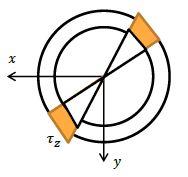
\includegraphics[width=0.5\linewidth]{immagini/screenshot001}
			\label{fig:screenshot001}
		\end{figure}
		
		
		I dati collezionati in questo diagramma hanno tuttavia poco senso, ci sono tanti dati ammucchiati intorno allo $ 0 $ e pochi dati caratterizzati da assenza di rottura questa tipologia di assali in particolare, caricati in maniera minore, duravano senza ma rompersi, evidenziando come al di sotto di una certa tensione non ci fossero effetti di fatica. \newline
		
		Ma cosa emerge riportando gli stessi grafici in forma semi logaritmica? 
		
		\begin{figure}[H]
			\centering
			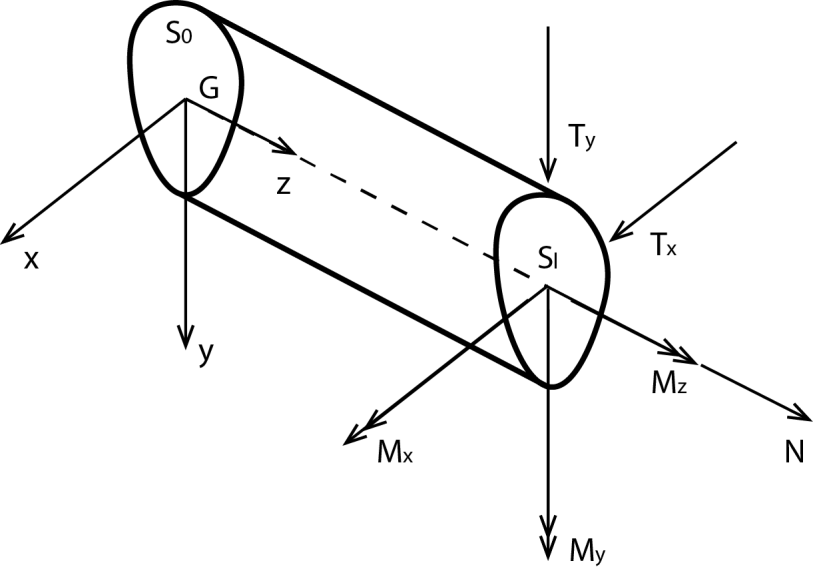
\includegraphics[width=0.5\linewidth]{immagini/screenshot002}
			\label{fig:screenshot002}
		\end{figure}		
		
		Improvvisamente i dati si vengono a correlare lungo una curva, ma se il grafico fosse allora doppio logaritmico?
		
		\begin{figure}[H]
			\centering
			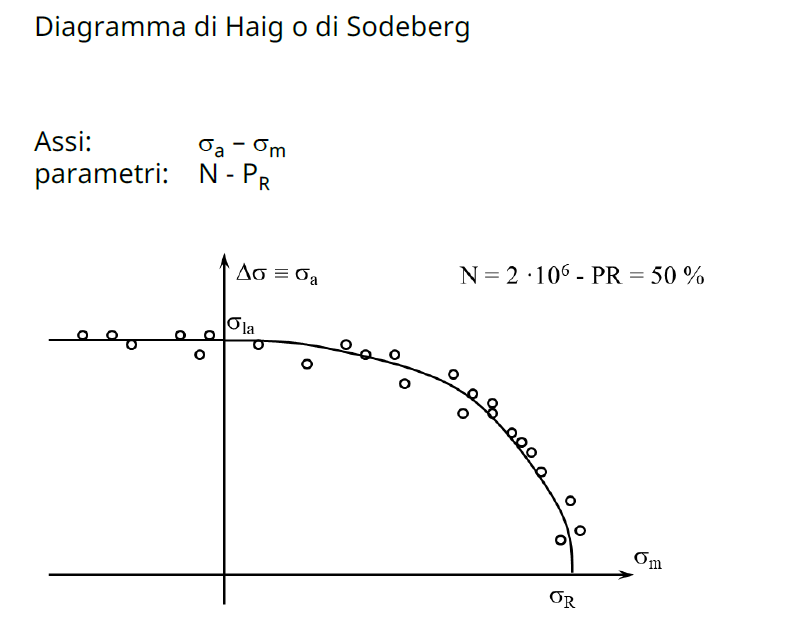
\includegraphics[width=0.5\linewidth]{immagini/screenshot003}
			\label{fig:screenshot003}
		\end{figure}		 
		
		Ecco così che i dati sperimentali si attestano lungo ad una retta. 
		
		Questa dispersione di dati rappresenta un valore limite (ginocchio della curva di Wöhler) al di sotto del quale non c'è limite di fatica: sotto a quel livello di carico il componente dura idealmente all'infinito. \newline
		
		Si può così considerare, per tutti i materiali che presentino questo ginocchio, una distribuzione doppio logaritmica  rettilinea che si traduce in una relazione del tipo:
		\[\sigma^cN=cost\]
		Poiché Wöhler ha fatto sperimentazione sulla flessione rotante e dunque su un'oscillazione ciclica del carico caratterizzata da tensioni massime e minime uguali in modulo ma opposte di segno (a valore medio nullo), $\sigma$ altro non è che la semi-ampiezza di sollecitazione, che nel caso di sigma media nulla corrisponde alla sollecitazione massima; $ c $ è un coefficiente in prima approssimazione legato alle caratteristiche del materiale, che subirà delle correzioni in funzione di tutti quei fattori che influenzano la durata a fatica di un componente; $ N $ è il numero di cicli di applicazione della sollecitazione periodica considerata. \newline 
		
		Porre tale relazione costante equivale a dire che i punti della detta curva sono tutti legati tra loro, in pratica vuol dire che la conoscenza di una coppia di valori $(N, \sigma)$ di un punto sperimentale e la pendenza della curva, permette di conoscere, entrando col numero di cicli previsto, qual è la tensione limite da dover considerare. \newline
		
		Purtroppo i dati sperimentali non si piazzano tutti perfettamente in linea creando quella precisa curva, in realtà esiste una forte dispersione statistica del dato sperimentale, questo soggetto ad una distribuzione gaussiana anche piuttosto importante secondo la variabile $ N $, questa caratterizzata da un'ampiezza decisamente superiore. 
		
		\begin{figure}[H]
			\centering
			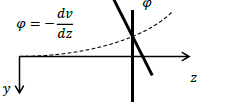
\includegraphics[width=0.5\linewidth]{immagini/screenshot004}
			\label{fig:screenshot004}
		\end{figure}
		
		In questo grafico reale si ritrova sicuramente il trend ritrovato Wöhler ma i punti ora non sono più perfettamente allineati, sostanzialmente la curva originale in azzurro delimita inferiormente o superiormente i dati sperimentali: tracciare una curva come in figura significa identificare una bassa probabilità che i dati sperimentali siano al di sotto e un'altissima probabilità che siano al di sopra, vuol dire che associata a quella curva c'è un'alta probabilità di sopravvivenza e una bassa probabilità di rottura. 
		
		Se quella curva la si utilizza come verifica di resistenza, c'è un'alta probabilità che il dato sperimentale caschi oltre, mentre una bassa probabilità che caschi al di sotto, è molto affidabile. 
		
		Le curve limite che si utilizzano per determinare i limiti di fatica sono quelle al 10\% e al 90\% della probabilità di rottura, due curve identificano un'area, l'80\% dei dati sperimentali. \newline
		


		Perché c'è così tanta dispersione? Il fenomeno della fatica a livello microscopico è estremamente complesso, prima di tutto perché sia la possibilità che si inneschi che la condizione per la quale si propaghi possiedono una loro probabilità, e poi c'è da considerare la probabilità legata al raggiungimento della condizione critica. \newpage
		
		
		\textbf{\Large Le fasi di Fatica} \newline
		La fatica si innesca in presenza di un qualunque tipo di difetto sulla superficie e questi, in casi reali, sono sempre presenti. La rottura per cricca di fatica si suddivide in tre fasi: l'innesco ( o nucleazione), la propagazione e il cedimento. \newline
		
		In una prima fase la cricca avanza all'interno del materiale, ad esempio nei materiali duttili a 45\degree rispetto alla direzione di carico, arrivata ad una certa profondità si propaga in direzione ortogonale alla direzione di applicazione del carico, fino a separare così tanta sezione resistente che quella rimasta non non diviene più staticamente più in grado di sorreggere il carico applicato. 
		
		\begin{figure}[H]
			\centering
			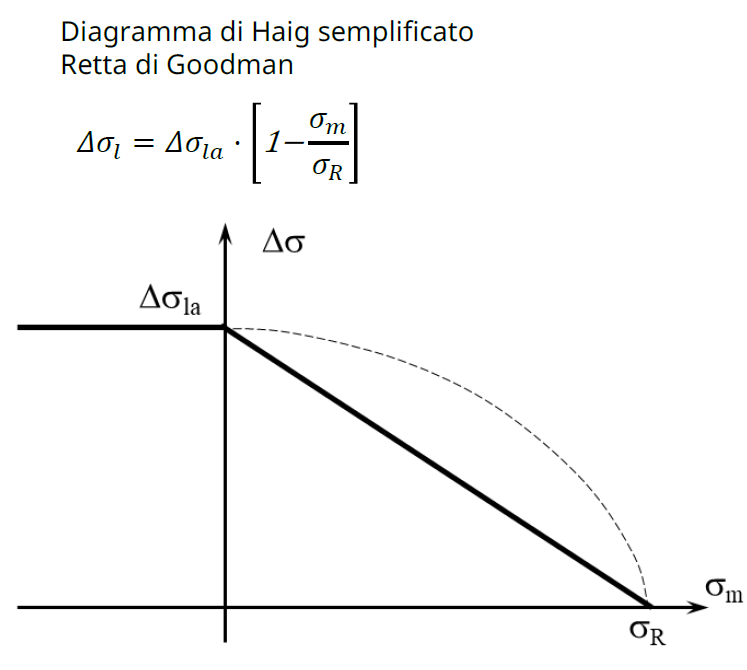
\includegraphics[width=0.5\linewidth]{immagini/screenshot005}
			\label{fig:screenshot005}
		\end{figure}
				
		Queste tre fasi lasciano sul materiale un'impronta tale che, se si dovesse analizzare la superficie di frattura si è chiaramente in grado di capire se la rottura è avvenuta staticamente o per fatica. La zona dell'innesco è frastagliata, talvolta più scura a causa dell'ossidazione e ha una forma irregolare, a partire poi dalla zona d'innesco, inizia la propagazione della cricca viaggerà lungo la sezione permettendo la visione del progressivo danneggiamento.
		
		\begin{figure}[H]
			\centering
			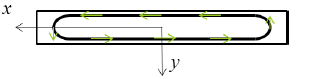
\includegraphics[width=0.5\linewidth]{immagini/screenshot006}
			\label{fig:screenshot006}
		\end{figure}		
		
		Su questo avanzamento si è in grado di notare esattamente delle linee di avanzamento, le striature di fatica, \textit{beachlines}, legate all'impronta che lascia la cricca ogni volta che avanza; questa infatti avanzando nel momento in cui si traziona il componente e arrestandosi quando lo si comprime, diviene facilmente distinguibile sul pezzo, inoltre, durante il processo di compressione, e dunque di chiusura della cricca le due superfici separate si lucidano dando alla sezione un aspetto lucido e liscio. Infine, quando la sezione resistente diviene oramai inadeguata a carico applicato, si romperà di schianto. \newline
		
		\textbf{Fase 1: innesco}\newline
		Fortunatamente le tre fasi non sono proporzionali l'una con l'altra in termini di vita del componente, la prima fase di nucleazione, ovvero la fase in cui un piccolo danneggiamento superficiale diventa un vero e proprio innesco della cricca, occupa solitamente l'80\% della vita del componente, il vero problema è che proprio l'innesco fa poi partire la fase di propagazione, questa nettamente più veloce. La condizione per la quale si distingue tra un innesco che ha fatto partire una cricca e un innesco che no è riuscito a far partire una cricca è legato ad una serie di fattori quali la dimensione dell'innesco, la capacità di resistenza all'innesco e il livello di carico. Si può benissimo avere un innesco che per tutta la vita del componente non parte così come un innesco magari più piccolo ma su di un materiale molto più sensibile che da vita alla propagazione di una cricca. 
	
		Raggiunta una determinata condizione di innesco, la fase di nucleazione si conclude e la
		cricca procede a 90\degree rispetto al carico. \newline
		
		L'innesco della frattura può avvenire per:
		\begin{itemize}
			\item Difetto locale sulla superficie;
			\item Zone di brusche discontinuità geometriche;
			\item Difetti interni considerevoli (soffiature)
			\item Zone attaccate chimicamente (presenza rugosità più accentuata)
			\item Tensioni residue considerevoli (dalle lavorazioni)
			\item Zone di contatto
			\item Inclusioni
		\end{itemize} 
	
		Talvolta non è un danno a cerare l'innesco, ma semplicemente lo scorrimento dei piani cristallini.
		
		In un materiale duttile soggetto a trazione si ha uno scorrimento dei pani cristallini a 45\degree, se questa sollecitazione diviene alternata, questi piani scorrono in una direzione e poi tornano indietro e dato che non riusciranno mai a re-impilarsi esattamente come prima,la superficie di bordo subisce una variazione di forma con sporgenze e rientranze. Sono queste variazioni a determinare una concentrazione di tensioni, un difetto superficiale che innescherà la cricca. 
		
		\begin{figure}[H]
			\centering
			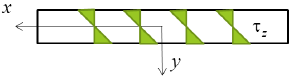
\includegraphics[width=0.25\linewidth]{immagini/screenshot007}
			\label{fig:screenshot007}
		\end{figure}		 
	
		Si è facilmente dimostrato come lappando il componente si allunga la sua vita utile a fatica. \newline
		
		\textbf{Fase 2: Propagazione}\newline
		L'innesco ora è caricato, è aperto, quando si scarica si richiude, richiudendosi l'apice della cricca diminuisce il suo raggio di curvatura: $K_t\rightarrow1000$, localmente si sta pasticizzando il materiale, ma in realtà è ben oltre la plasticizzazione, si arriva  alla rottura locale del materiale, sono che essendo circondato da materiale ancora in condizione plastica non avviene una propagazione per tutta la sezione ma una rottura locale con plasticizzazione della zona subito adiacente, quando si va a riaprire, a ricaricare, a trazionare la cricca, si ha una nuova separazione dei due lembi con il conseguente avanzamento dell'apice: ad ogni ciclo di trazione compressione, la cricca avanza.
		\begin{figure}[H]
			\centering
			\begin{subfigure}{0.5\textwidth}
				\centering
			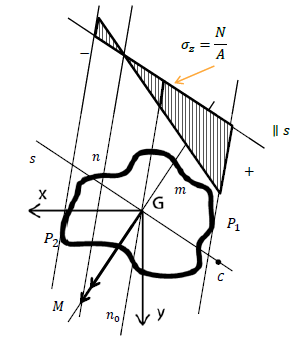
\includegraphics[width=\linewidth]{immagini/screenshot008}
\label{fig:screenshot008}
			\end{subfigure}%
			\begin{subfigure}{0.5\textwidth}
				\centering
			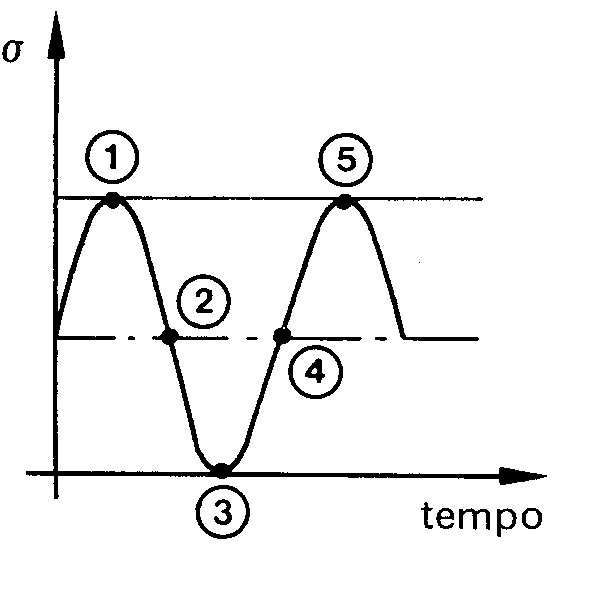
\includegraphics[width=\linewidth]{immagini/screenshot009}
\label{fig:screenshot009}
			\end{subfigure}
		\end{figure}
		
		La legge temporale con cui avanza, ovvero la sua velocità di avanzamento, è definibile tramite la meccanica della frattura attraverso la relazione di Paris. Tale velocità di propagazione è elevatissima, centinaia di metri al secondo. A seguito del carico, quando l'innesco è sufficiente per far avanzare la cricca, molto spesso è ormai troppo tardi, in  pochissimi cicli la cricca si è propagata e ha ridotto la sezione resistente fino alla rottura di schianto. 
		
		In termini di  ogni ciclo, l'avanzamento  varia da $10^{-4}\div0.1 mm/ciclo$. 
		
		A quanti giri al minuto va un albero motore di una vettura? $ 500giri/s $, se la cricca avanza di $ 0.1 mm $ a giro avanza di $ 50 cm/s $ ed in meno di mezzo secondo l'albero è distrutto. 
		
		Non c'è dunque un modo di monitorare in certe applicazione l'avanzamento di una cricca, c'è solo da far prevenzione nel ridurre la probabilità dell'avere degli inneschi sufficientemente grandi da non far partire questa cricca.\newline  
		
		\textbf{Fase 3: Rottura di Schianto} \newline
		Quando la propagazione indebolisce la sezione resistente al punto che la superficie residua non è più sufficiente a sopportare il carico massimo applicato il componente cede di schianto, senza preavviso.
		
		La modalità di frattura può essere sia duttile che fragile, dipendentemente dal materiale, dal livello di stress, dall'ambiente circostante ecc\dots
		
		La dimensione, la forma e la localizzazione della rottura sono elementi fondamentali per l'analisi delle cause che hanno portato al collasso l’elemento. "Leggere" una rottura di fatica è essenziale per evitare il ripetersi del fenomeno. \newline
		
		\textbf{\Large Caratteristiche della frattura per fatica} \newline
		Per quanto visto finora risulta quindi relativamente semplice identificare una rottura per fatica.
		
		Infatti, mentre l'aspetto microscopico è transgranulare, a livello macroscopico e piatta e regolare. 
		
		Nella porzione di sezione sede della propagazione vi è la presenza di una serie di striature, rughe, avvallamenti, cretti. Il passo tra due striature consecutive è piccolo nella fase iniziale dove la cricca si propaga lentamente e aumenta quando la riduzione dell’area resistente fa aumentare lo sforzo applicato e la cricca si propaga velocemente. 
		
		\begin{figure}[H]
			\centering
			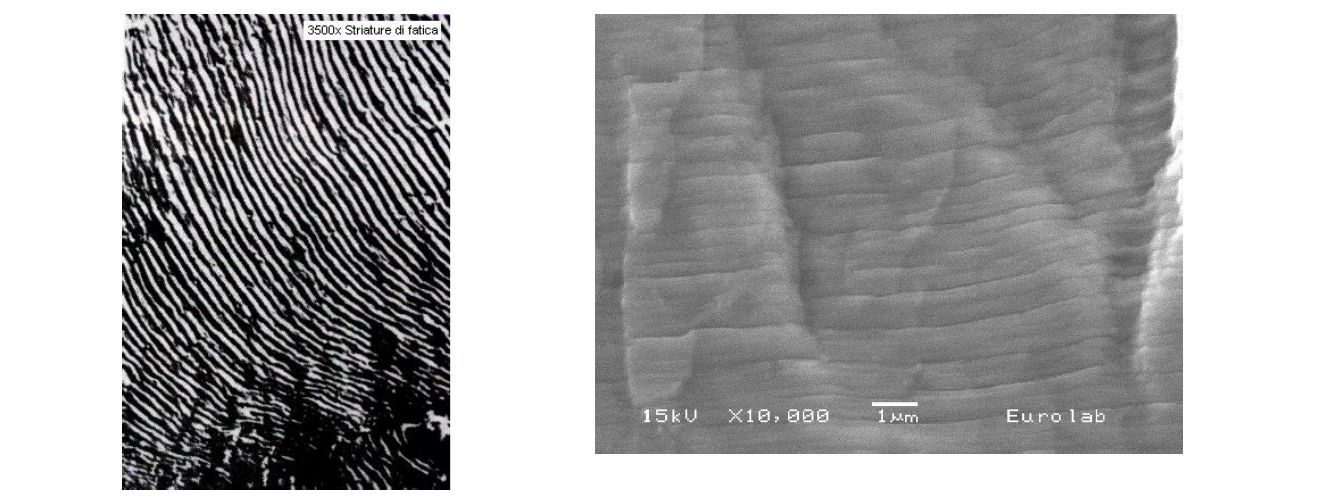
\includegraphics[width=0.5\linewidth]{immagini/screenshot010}
			\label{fig:screenshot010}
		\end{figure}		
		
		Dato che l'innesco di una frattura per fatica non richiede uno sforzo elevato, la deformazione plastica - durante la fase di propagazione - è presento solo all'apice della cricca ed è perciò relegata ad una zona di estensione modesta. 
		
		Le deformazioni plastiche saranno quindi presenti nella sola zona di rottura finale, dove il meccanismo sarà analogo a quello che si verifica nella parte finale di una prova statica. In questa zona l’entità delle
		deformazioni dipende dalla duttilità o fragilità del materiale.
		
		 \end{adjustwidth}
		\begin{figure}[H]
		\includegraphics[scale=0.75,page=19]{10_fcm_2022}
		\end{figure}
		\begin{adjustwidth}{2in}{}
		
		Ad esempio, ricordi he per torsione le tensioni sono massime sul bordo esterno della sezione? In questo caso la cricca non avanzerà molto l'interno ma interesserà maggiormente le parti periferiche della sezione. \newline
		
		Ogni punto della curva di Wöhler racconta una storia. 
		\begin{figure}[H]
			\centering
			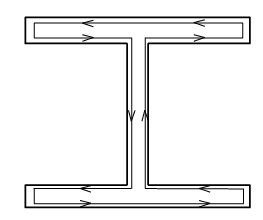
\includegraphics[width=0.5\linewidth]{immagini/screenshot011}
			\label{fig:screenshot011}
		\end{figure}
		
		Quando ci si trova ad evidenziare la rottura di un componente, quel componente durante la sua storia di carico ha dapprima subito una prima iniziale dove i difetti, le cricche, sono estremamente piccole e visibili solo al microscopio, poi una fase in cui le cricche divengono visibili e poi ancora una possibile situazione dove queste condizioni si sommano tra loro portando un avanzamento più veloce che conduce alla la propagazione e poi all'inevitabile frattura.
		
	\end{adjustwidth}
	\begin{figure}[H]
	\includegraphics[scale=0.75,page=24]{10_fcm_2022}
	\end{figure}
	\begin{adjustwidth}{2in}{}
		
		Per  livelli di carico più bassi non c'è sostanzialmente sufficiente energia per far propagare le cricche che si estendono sulla sezione, e quindi all'avanzare del numero di cicli le cricche rimangono ferme: non c'è sufficiente energia di deformazione per farle avanzare. \newline   
		
		\textbf{\Large Tipi di cicli di sollecitazione} \newline
		Quali sono gli elementi che vanno a influenzare la fatica e cosa determina l'insorgenza delle criticità?
		
		Ricapitolando, la fatica è un fenomeno che si manifesta esternamente attraverso una frattura fragile istantanea che avviene a seguito dell'applicazione di carichi ciclici, ripetuti, con entità del carico massimo anche piuttosto bassa rispetto ai limiti statici di snervamento. 
		
		La semplificazione che si andrà a fare nel trattare questo fenomeno sarà quella di valutare una condizione del tutto ideale nella quale i carichi siano perfettamente ciclici, o comunque, nella loro ciclicità abbiano un andamento sinusoidale. \newline
		
		In realtà lo studio con questo approccio deriva dalle prime evidenze sperimentali nelle quali  effettivamente si studiava proprio una sollecitazione ciclica con andamento temporale sinusoidale: l'andamento della $ \sigma_z $ su un elemento cilindrico sottoposto a flessione rotante (assale di Wöhler) è proprio un andamento sinusoidale della tensione nel tempo, con massimo, minimo e valore medio nullo.
		
		La sollecitazione di flessione rotante è proprio quella sollecitazione descritta da un momento flettente costante in direzione modulo e verso ma applicata ad un elemento cilindrico rotante, di conseguenza la tensione è ciclica a fronte di una sollecitazione costante.  \newline
		
		Nella realtà si è in grado di schematizzare il tipo di ciclo di sollecitazione in funzione di due o tre parametri caratteristici. Stante l'ipotesi di una tensione che varia con legge sinusoidale, quindi con ampiezza e periodo costanti nel tempo, si dovrà fissare la tensione massima e quella minima o la tensione media ed una semiampiezza di sollecitazione per conoscere il ciclo di sollecitazione: i parametri di riferimento saranno sempre le due coppie di valori appena citate.
		\begin{figure}[H]
			\centering
			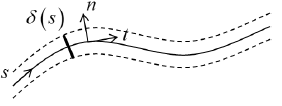
\includegraphics[width=0.5\linewidth]{immagini/screenshot012}
			\label{fig:screenshot012}
		\end{figure}
		
		La semiampiezza altro non è che:
		\[\sigma_a\dfrac{\sigma_{\max}-\sigma_{\min}}{2}\]
		
		Si conclude così che una coppia di valori di tensione fornisce uno spettro di carico. \newline 
		
		Un altro parametro interessante per classificare i tipi di cicli di sollecitazione è il rapporto di ciclo
		\[R= \dfrac{\sigma_{\min}}{\sigma_{\max}}\]
		
		\textbf{$ R = -1 $} è una sollecitazione di flessione rotante. 
		
		Qual era la caratteristica del grafico di Wöhler in condizioni standard? Di avere $\sigma_m  = 0$. 
		In quel diagramma nelle ordinate si metteva la semiampiezza di sollecitazione $\sigma_a$ relativa ad un ciclo a tensione media nulla, perciò per andare a individuare esattamente un diagramma standard di sollecitazione basta dire o che la tensione media è nulla o che il rapporto di ciclo è uguale a $ -1 $. 
		
		\textbf{$R=0$} indica una sollecitazione di pulsazione di trazione, una sollecitazione che va parte da 0 e arriva ad un valore di trazione. 
		
		\textbf{$R=1$} non è un carico ciclico, è un carico costante, è la condizione di sollecitazione statica.
		 
		\textbf{$R=\pm\infty$} è caratterizzato dall'avere una massima nulla ed una minima non nulla, e poiché per definizione la minima avrà valore negativo, sarà condizione di pulsazione dallo 0 di compressione. \newline
		 
		Come identificare un ciclo che non ha questi valori determinati? Analizzando la sollecitazione.
		
		Innanzitutto se questa fosse mista trazione-compressione il rapporto di ciclo avrebbe un segno meno ed un valore compreso tra 0 ed 1 quindi è sola trazione: i rapporti con segno meno davanti indicano che le tensioni massime e minime sono discordi le la sollecitazione sarà mista. 
		
		Perciò per avere la sola compressione dovrà essere $R>1$, la minima e la massima saranno entrambe negative e il rapporto ci ciclo sarà positivo con minima in modulo maggiore della massima. \newline
		 
		Con queste classificazioni si indicano i tipi di sollecitazione, ma perché è importante indicarlo?
		
		È il rapporto di ciclo ad influenzare la durata a fatica del componente, incida il processo di avanzamento delle cricche, queste infatti si aprono a trazione, mentre a compressione si richiudono, e poiché si quantifica la vita a fatica del componente in funzione del numero di cicli di carico che questo è in grado di sopportare, sarà proprio la quantità di cicli di trazione a fare allora la differenza di durata di un componente. \newline
		 
		Infatti nei diagrammi di rappresentazione della fatica non basta mica indicare media e semiampiezza ma si devono aggiungere altri due termini, come la durata $ N $ di giri e probabilità di accadimento di un evento, di rottura.
		 
		Questi quattro parametri sono esattamente quelli che servono per identificare una condizione di criticità.
		
		Il fatto però di avere 4 parametri e di lavorare con rappresentazioni di tipo cartesiano a due variabili, impone che la rappresentazione della condizione di criticità a fatica avvenga utilizzandone due mentre gli altri verranno fissati ad un valore di riferimento. Esempio tipicissimo è proprio il diagramma di Wöhler, in ascissa c'è il numero di cicli e in ordinata la semiampiezza mentre vengono fissate un certo valore di probabilità di rottura ed un certa tensione media (nulla). \newline
		 
		Dov'è che però si ha difficoltà nell'interpretazione pratica di questi grafici? 
		
		Per prima cosa le sollecitazioni nella realtà speso non sono monodimensionali, mentre nel diagramma c'è una semiampiezza: la fatica è studiata in condizioni monodimensionali ma nella realtà è un problema tridimensionale.
		
		Un'altra difficoltà è legata alla combinazione di cicli, questi di solito non hanno una forma regolare e sinusoidale, ma possono avere una certa non-stazionarietà, per cui solo con forte approssimazione sono perfettamente costanti in ampiezza e periodo nel tempo. 
		
		Non si può poi non considerare il valore di tensione media, questa infatti altera importantemente la durata a fatica di un componente, tant'è che il diagramma standardizzato così com'è non può essere utilizzato in presenza di $\sigma_m\ne0$.
		
		Infine sussiste anche una certa complessità nel valutare la durata di un componente quando si susseguono cicli di carico con frequenze differenti: la storia di carico influenza anch'essa la durata a fatica. Questo lo si può già immaginare ricordando il meccanismo che porta alla rottura, se si sta sollecitando un pezzo e questo comincia a presentare delle cricche durante la trazione, non è più come sollecitare un componente elasticamente per cui non importa della sua storia di carico finché questo non abbia raggiunto il suo valore limite, in realtà nella fatica ogni ciclo di sollecitazione sta apportando un danneggiamento. Infatti se ad esempio si sollecita un componente a bassi livelli di tensione, questi, incapaci di aprire una cricca non sortiranno alcun effetto al materiale, se poi a questi livelli si susseguono tensioni già più importanti che riescono ad aprire una cricca, il componete giungerà a rottura ma solo con questo nuovo treno di sollecitazioni. Al contrario, applicando subito una tensione considerevole facendola seguire da una più moderata, non importerà più che quella nuova sia minore della precedente, se la cricca è già formata il componente arriverà a rottura ugualmente anche per tensioni più piccole. \newline
		 
		L'approccio alla fatica può avvenire così in modi differenti, in questa trattazione si userà il \textit{Safe Life}: si predirà la durata a fatica del componente soggetto a quella sollecitazione. Altri approcci che si basano sul \textit{Fail Safe} cioè sull'andare a capire cosa accade nel caso di cedimento a fatica. Un altro approccio è fornito dal \textit{Damage Tolerance}, è l'approccio tipico della meccanica della frattura, è una modellizzazione del fenomeno che pone l'attenzione proprio sul monitorare tutto ciò che accade tra l'innesco e il cedimento, dalla nascita della cricca all'avanzamento in tempo reale della stessa. \newpage
		
		\textbf{\Large Caratteristiche di cicli} \newline		 
		La prima cosa che deve essere  approfondita è legata ad una serie di considerazioni da fare sul ciclo reale di carico, nella realtà come detto questi non sono affatto perfettamente sinusoidali, ma sono spettri di carico ad ampiezza, frequenza e sforzo medio non costante. 
		
		Ora, dato che si vuole trovare una corrispondenza tra teoria e realtà con approcci semplificativi e quindi con modelli equivalenti da applicare al caso reale, si è nella condizione di ricercare un ciclo di carico che per quanto irregolare nel tempo e complesso da analizzare sia, presenti lo stesso in qualche modo una ripetibilità temprale, d'altronde solo in presenza di ciclicità si manifesta la fatica, dato poi che questa si manifesta a $10^4$ cicli, un'altra condizione che deve rispettare il ciclo di carico è quello di essere sufficientemente ripetuto.
		
		\begin{figure}[H]
			\centering
			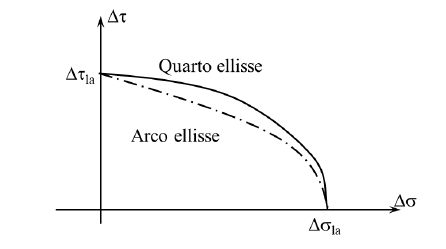
\includegraphics[width=0.5\linewidth]{immagini/screenshot013}
			\label{fig:screenshot013}
		\end{figure}
		 
		 Varrebbe in questo caso un'analisi dello spetto con Fourier? D'altro canto una qualunque curva nel tempo si può ridurre ad una combinazione di lineare di funzioni sinusoidali ma su che concetto si basa la trasformata di Fourier? Questa è basata sulla combinazione in frequenze di seni e coseni a diversa ampiezza e fase, nella fatica si lavora solo con fase zero mentre tutti i cicli di carico devono avere lo stesso periodo, l'unica cosa su cui si può lavorare rimane l'ampiezza della sollecitazione. 
		 
		 Nella fatica la funzione sinusoidale si può distinguere solo in ampiezza, mentre non può essere manipolata nè in forma, nè in periodo e nè in fase.\newline
		  
		 \textbf{Metodo del serbatoio}\newline
		 Molto pratico, permette il calcolo di un certo numero di cicli equivalenti che abbiano lo stesso effetto del ciclo reale.
		  
		 \begin{figure}[H]
		 	\centering
		 	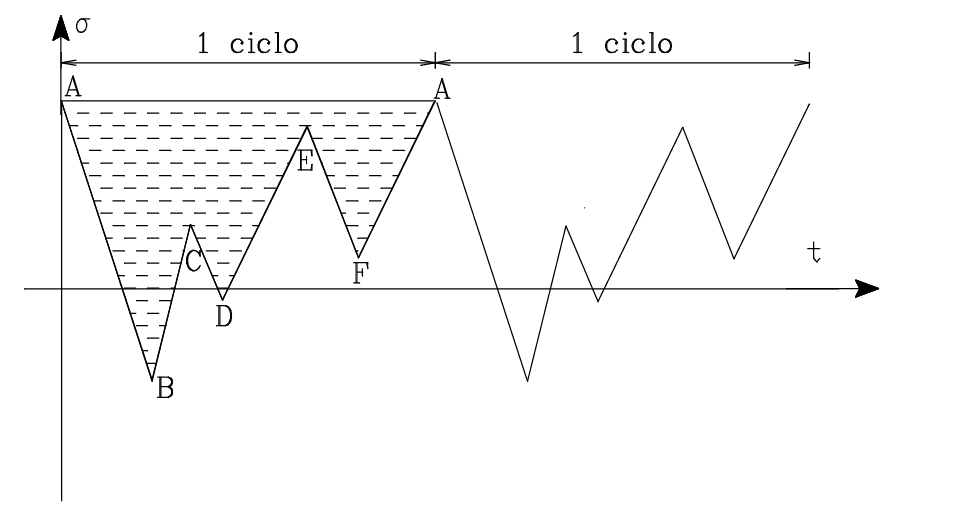
\includegraphics[width=0.5\linewidth]{immagini/screenshot014}
		 	\label{fig:screenshot014}
		 \end{figure}
		 		  
		 Si riempia il grafico con acqua, a seguito del riempimento si stappi il minimo dei minimi, svuotando il serbatoio dove rimane l'acqua? Nelle valli, laddove si avranno delle valli ben definite caratterizzate da valori massimo e minimo, quello sarà il ciclo di carico. Reiterando il processo e stappando tra più cicli sempre il minimo dei minimi, quello che si ottiene infine è una successione di cicli di carico che sommati insieme procurano lo stesso danneggiamento a fatica del ciclo reale.
		 
		 \end{adjustwidth}
		 \begin{figure}[H]
		 \includegraphics[scale=0.75,page=30]{10_fcm_2022}
		 \end{figure}
		 \begin{adjustwidth}{2in}{}
		 
		 Questo metodo permette di individuare tutta una serie di cicli caratterizzati da diverse semiampiezze e valori medi. 
		  
		 Esistono metodi più semplici, mono-parametrici, in cui si individua di volta in volta la semiampiezza di ciascun ciclo. I cicli che si vanno così ad individuare hanno in comune la medesima tensione media e differiscono l'uno dall'altro dal solo valore di semiampiezza. \newline
		 
		 \textbf{Peak Counting}\newline
		  Il metodo del Peak Counting consiste nel calcolare la tensione media del ciclo.
		  
		  \begin{figure}[H]
		  	\centering
		  	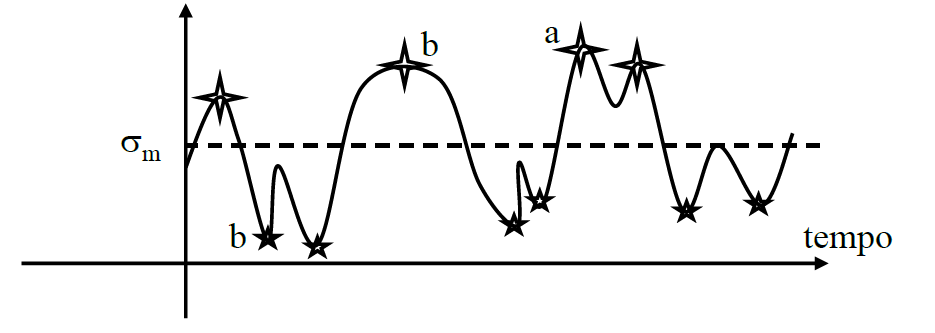
\includegraphics[width=0.5\linewidth]{immagini/screenshot015}
		  	\label{fig:screenshot015}
		  \end{figure}
		  
		  
		  Si attribuisce una tensione media e si dividono i minimi coi massimi in un processo in cui il massimo dei massimi viene abbinato al minimo dei minimi a seguire.
		  Accoppiando a due a due i picchi si ottiene un certo numero di cicli equivalenti ognuno di semiampiezza pari a
		  \[\sigma_a = \dfrac{\sigma_{\max}-\sigma_{\min}}{2}\]
\newpage		  
		  \textbf{Level Crossing}\newline
		  In questo metodo si individua la media del ciclo e si isola un nuovo sotto-ciclo ogni volta che la retta del valore medio interseca due volte il ciclo di partenza, proprio come se fosse un periodo, il sotto-ciclo sarà così caratterizzato da una semiampiezza pari a
		  \[\sigma_a = \dfrac{\sigma_{\max}-\sigma_{\min}}{2}\]
		  \begin{figure}[H]
		  	\centering
		  	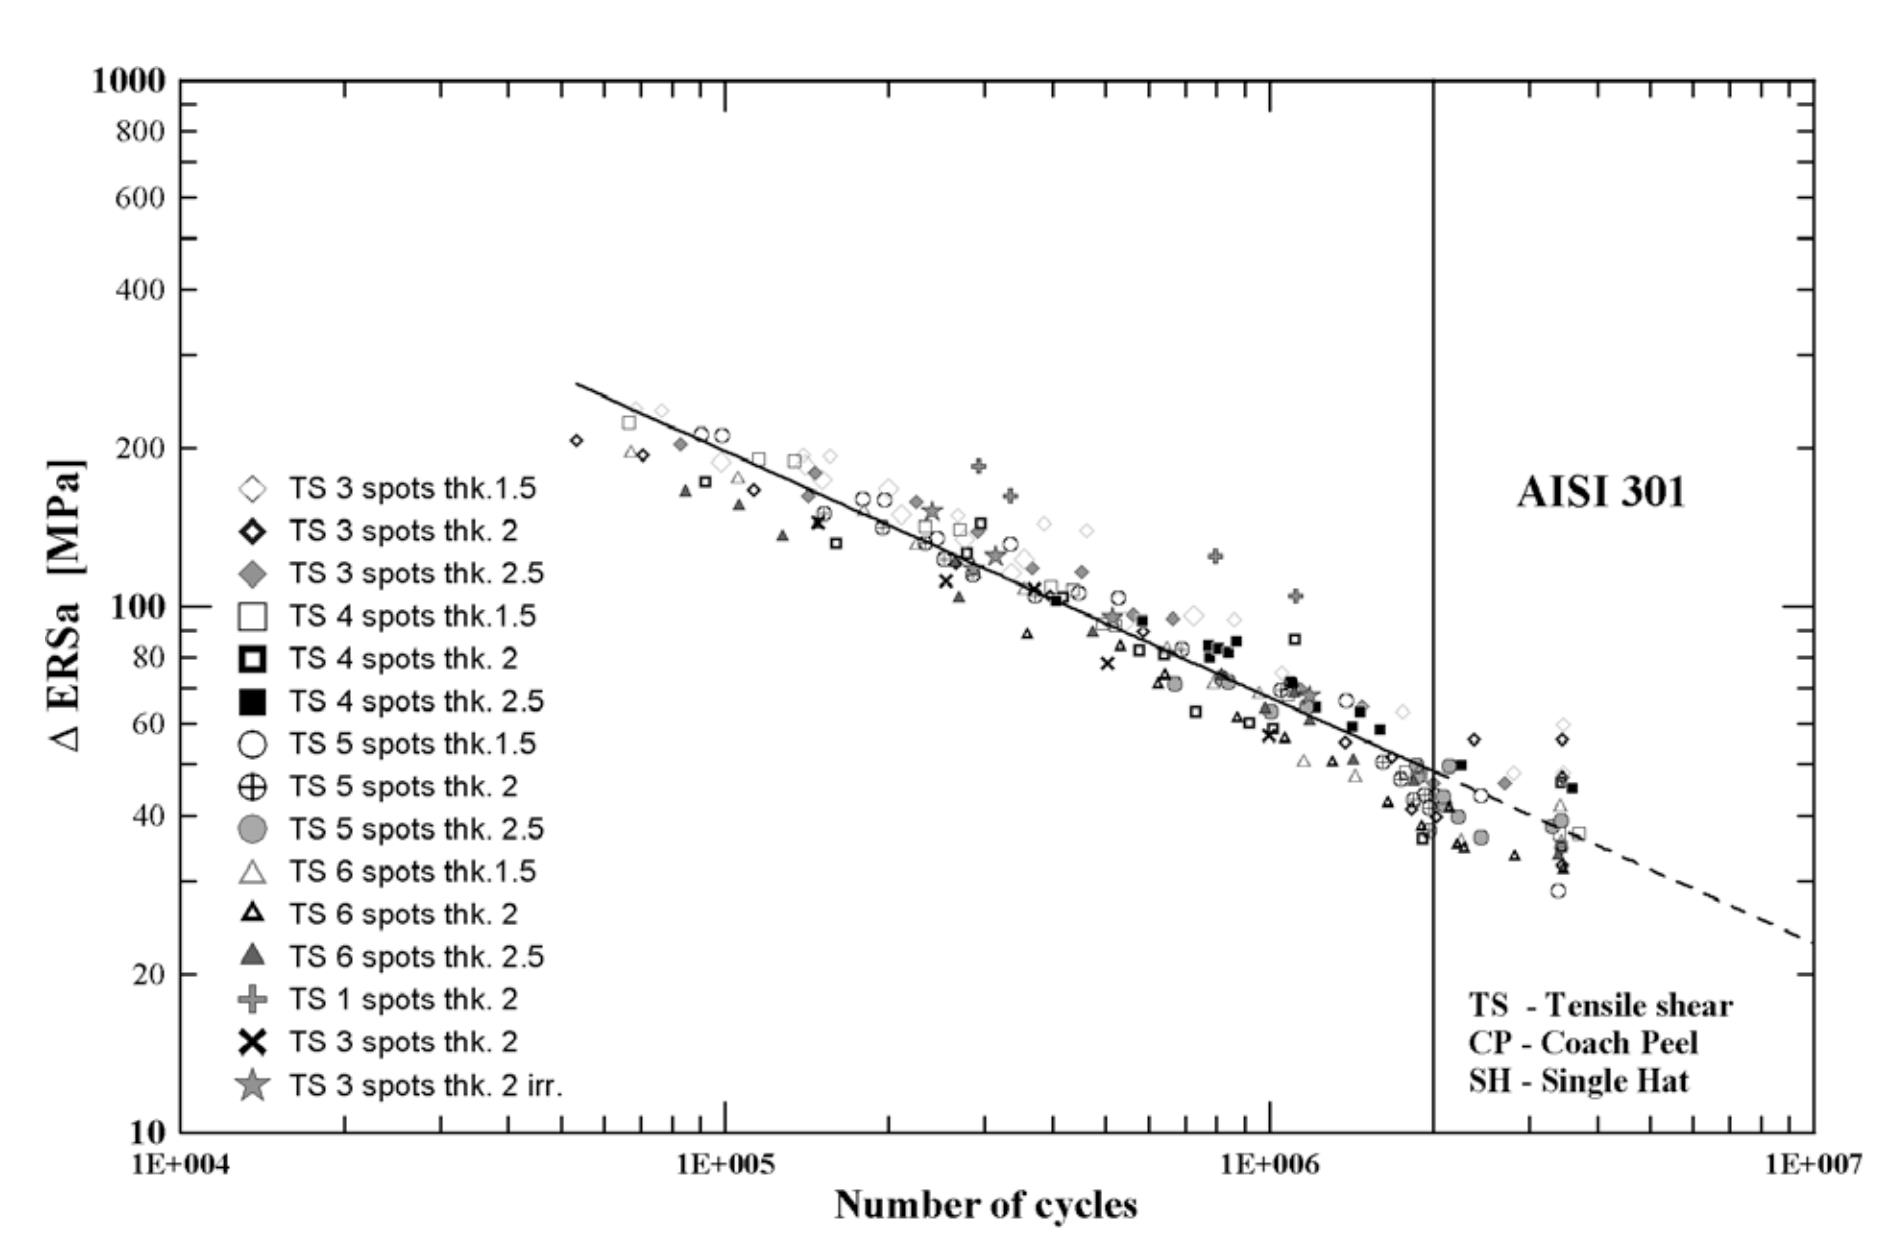
\includegraphics[width=0.5\linewidth]{immagini/screenshot016}
		  	\label{fig:screenshot016}
		  \end{figure}
		  
		  
		  \textbf{Range Counting}\newline
		  Oltre al metodo del serbatoio esistono metodi bi-parametrici come il \textit{Range Counting} in cui ogni coppia locale massimo-minimo contigua, in successione, accoppiata insieme, fornisce un valore medio e un valore di semiampiezza. 
		  \[\sigma_a = \dfrac{\sigma_{\max}-\sigma_{\min}}{2}\hspace{1cm} \sigma_m = \dfrac{\sigma_{\max}+\sigma_{\min}}{2}\]
		  Ogni coppia massimo - minimo contigua costituisce un mezzo ciclo. 
		  \begin{figure}[H]
		  	\centering
		  	
\includegraphics[width=0.5\linewidth]{immagini/screenshot019}
		  	\label{fig:screenshot019}
		  \end{figure}
		  
		  Questi sono solo una manciata di metodi che sperimentalmente funziona, riescono a ricavare un numero di cicli equivalente che abbia lo stesso apporto di danneggiamento del ciclo reale, per poterlo utilizzare manca però una legge di accumulo del danneggiamento, questa infatti sarà in grado di quantificare quando ciascun ciclo influenzi il danneggiamento del componente rispetto ad una criticità finale del componente stesso. \newline
		  
		  \textbf{\Large Prove di fatica} \newline 
		  Quanto si è appena visto vale per la modellizzazione della tensione applicata sul componente. 
		  
		  Come tutte le verifiche ingegneristiche è però necessario confrontare una grandezze d'esercizio con una caratteristica di resistenza del componente per quella determinata sollecitazione.
		  
		  La resistenza a fatica di un materiale non fa eccezione dalle prove statiche e si testa anch'essa in laboratorio.
		  
		  Le prove saranno ovviamente cicliche per questo più onerose di quelle statiche: non è economico provare un ginocchio a $2\cdot10^6$ cicli: una prova di fatica occupa per moto tempo le macchine operatrici.
		  
		  Tali macchine dovranno poi rispondere anche ad esigenze particolari di carico, queste infatti devono caratterizzare trazione e compressione in rapida successione sempre sotto le ipotesi di basse frequenze di applicazione per evitare l'instaurarsi di effetti dinamici, deve valere ciò che l'applicazione del carico non sia altro che l'applicazione statica di una successione di sollecitazioni, e quindi l'applicazione del carico non può non avvenire a basse velocità, per quanto questa risulti bassa però non è tuttavia attuabile mediante le classiche macchine di trazione note: le macchine di fatica sono estremamente più costose. 
		  
		  Dato inoltre che il tipo di sollecitazione modifica completamente la durata a fatica del componente, si avrà la necessità di macchine ce riescano a caratterizzarlo a sforzo normale, a flessione piana (flessione variabile nel tempo con pezzo fermo = sollecitazione variabile e tensione variabile), a flessione rotante, a torsione e a sollecitazione multiassiale. \newline
		  
		  In più, siccome il problema della fatica è affetto da una grande dispersione statistica - molto più di quella associata al problema statico -, per avere dei valori di riferimento si ha la necessità di una standardizzazione delle prove: la prova di caratterizzazione a fatica deve rispondere il più possibile a un certo numero di standard, solo in questo modo si è in grado di esporre e tabulare una resistenza legata il più possibile a quella del materiale.\newline
		  
		  Per fare un parallelismo con la verifica statica, questa prevedeva infatti che a destra della disuguaglianza ci fosse una tensione limite per quel componente in condizioni statiche e quella tensione limite era proprio quella del materiale, ovvero quanto questo potesse sopportare quel carico statico al netto di fattore di sicurezza, ora invece nella sollecitazione di fatica il termine che sta a destra della disuguaglianza è un termine che viene fortemente influenzato da tanti altri parametri oltre che dal materiale. 
		  
		\end{adjustwidth}
		\begin{figure}[H]
		\includegraphics[scale=0.75,page=35]{10_fcm_2022}
		\end{figure}
		\begin{adjustwidth}{2in}{}
		  
		  Per una flessione rotante creo uno schema statico appoggio-appoggio con il carico concentrato in due punti ricalcando esattamente l'assale di Wöhler, in questo modo il provino è caricato con momento flettente costante nel tempo e costante lungo il suo asse, questo, poiché ruoterà sperimenterà così una tensione variabile.
		  
		  Questa modalità di carico è molto comune ma ha uno svantaggio, applicando un momento flettente si ha una tensione sul pezzo e si legge quanti cicli è stato in grado di sopportare prima di rompersi, vuol dire che per ricreare un curva di Wöhler bisogna avere tanti provini quante tensioni è necessario testare. \newline 
		  
		  Ad un altro approccio si perviene utilizzando un provino sagomato a cui è applicato un carico a sbalzo, in queste condizioni si ha incastro e carico a sbalzo,è una mensola il cui momento flettente costante nel tempo ma linearmente variabile lungo il suo asse, in queste condizioni ciascuna sezione è sollecitata ad un diverso e determinato livello di carico. Questo è un metodo più flessibile. \newline
		  
		  \textbf{Criteri di classificazione delle macchine di prova} \newline
		  Si classificano le prove di fatica in base al tipo di carico applicato, alla modalità di variazione delle sollecitazioni e alla tipologia di pezzo in prova:
		  
		  Se una prova su di un provino standard la svolge l'ente certificatore, durante una fase di prototipazione e per determinati componenti che hanno urgenze di affidabilità o prestazione la prova di fatica si fa direttamente sul prototipo del componente, come ad esempio nel caso delle sospensioni automobilistiche.
		  
		  Si identificano quindi i seguenti criteri:
		  
\begin{figure}[H]
	\centering
	\begin{subfigure}{0.5\textwidth}
		\centering
		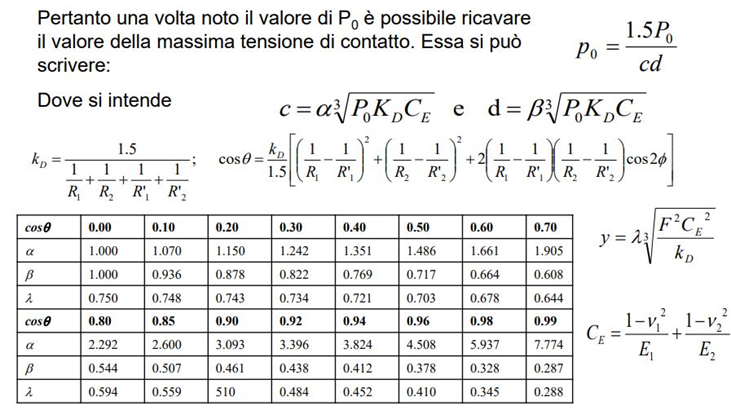
\includegraphics[width=\linewidth]{immagini/screenshot017}
		\label{fig:screenshot017}
	\end{subfigure}%
	\begin{subfigure}{0.5\textwidth}
		\centering
		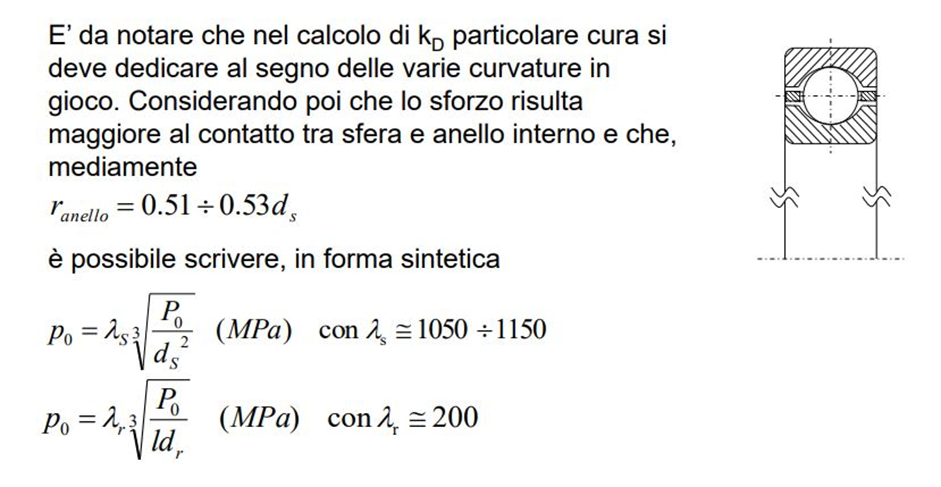
\includegraphics[width=\linewidth]{immagini/screenshot018}
		\label{fig:screenshot018}
	\end{subfigure}
\end{figure}
		  			  
		  Si riportano poi lo schema di funzionamento di una macchina idraulica e di un vibroforo, nel caso del vibroforo un eccitatore ed una molla producono una serie di vibrazioni sul componente. 
		  
		  		\end{adjustwidth}
		  \begin{figure}[H]
		  \includegraphics[scale=0.65,page=38]{10_fcm_2022}
		  \end{figure}
		  \begin{adjustwidth}{2in}{}
		  
		  \textbf{Come si svolge un campionamento a fatica? } \newline		  
		  Si fanno prove orientative su un numero ridotto di provini ognuno caratterizzato da una certa quantità di valori dello sforzo agente così da avere l'ordine di grandezza del numero di cicli di rottura, dato che poi si dovrà comunque avere una certa consistenza statistica, in funzione del livello di carico si dovrà prevedere una certa numerosità di prove dato che la singola prova di fatica non sarà mai sufficiente.

		  Si raccolgono poi le numerosità in funzione dei cicli di rottura. La curva di Wöhler è quella che racchiude per ciascun livello di carico o il 10\% o il 50\% o il 90\% di questi provini, la coppia (carico applicato, numero di cicli) che si trova sulla curva $\sigma^cN=cost$ nel diagramma doppio logaritmico di Wöhler è ad esempio caratterizzata da un certo livello di probabilità.
		  
		  \begin{figure}[H]
		  	\centering
		  	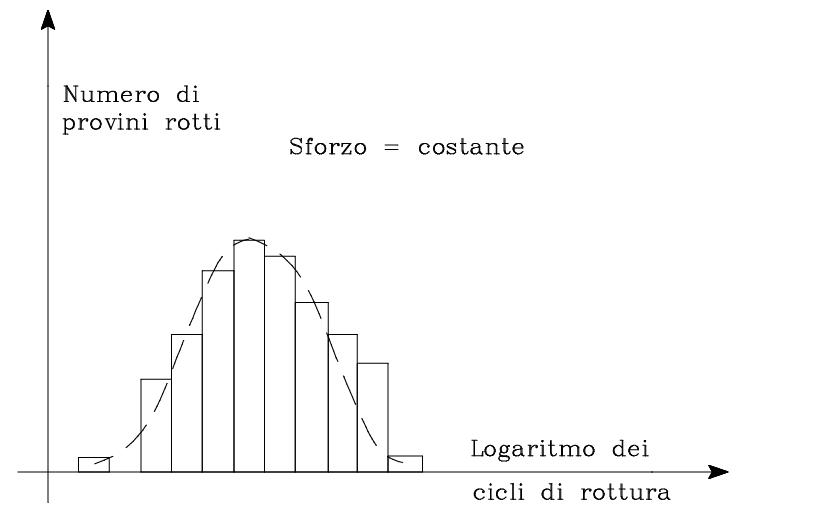
\includegraphics[width=0.5\linewidth]{immagini/screenshot020}
		  	\label{fig:screenshot020}
		  \end{figure}
		  
		  \textbf{\Large Parametri che influenzano la vita a fatica} \newline 		  
		  I parametri di cui è necessario tener conto per stabilire la vita a fatica di un componente (non più del materiale) sono suddivisibili in interni ed esterni. 
		  
		  Quelli interni sono specifici del componente, quelli esterni sono dettati dalle condizioni di utilizzo del componente. \newline
 			
 		  \textbf{Parametri Interni:} 
 		  \begin{itemize}
 		  	\item Materiale;
 		  	\item Finitura superficiale. D'altronde è da lì che partono le cricche; 
 		  	\item Tensioni residue dovute alle lavorazioni del componente;
 		  	\item Dimensioni. Delle sollecitazioni statiche non si è mai parlato della dimensione assoluta della trave, al massimo si è parlato di proporzioni, di snellezza, di quantificare una sezione rispetto alla lunghezza; a fatica le dimensioni influenzano la durata del componente;
 		  	\item Fattore di forma. Si era detto che per i materiali duttili la $K_t$ di concentrazione delle tensioni in condizioni statiche non si prende in considerazione, in condizioni di fatica la concentrazione di tensione dovute al fattore di forma è invece estremamente importante;
 		  	\item La corrosione è un parametro a cavallo tra interni ed esterni, è legata al livello di corrosione del componente ma è dovuta a condizioni ambientali di esercizio;
 		  \end{itemize}
 		  
 			\textbf{Parametri esterni:}
 			\begin{itemize}
 				\item Tipo di sollecitazione agente. Flessione rotante, trazione, flessione perfettamente alternata\dots 
 				\item Ciclo di sollecitazione> tutta trazione, tutta compressione o alternato; 
 				\item Frequenza del carico. Sotto una certa frequenza di carico esiste la fatica, al di sopra una si entra nel modo della dinamica;
 				\item Anche la resistenza a fatica come la resistenza statica è influenzata dalla temperatura;
 				\item Tensioni residue legate a sollecitazioni di utilizzo, alla storia di carico del pezzo. Ad esempio se il componente ha lavorato in condizioni plastiche per un po' e poi ritorna in fase elastica, le tensioni residue che si sono instaurate possono portare ad un'accelerazione della durata a fatica;
 				\item Saldature. La stragrande maggioranza dei componenti cede per fatica sulle saldature, sono delle zone di debolezza del componente;
 				\item Presenza di sollecitazioni multiassiali. Il problema tridimensionale influenza notevolmente la durata, è la frontiera di ricerca nell'ambito della fatica;
 			\end{itemize} 
 			\vspace{0.5cm}			
			\textbf{\Large Effetti legati al materiale} \newline
			La durata a fatica di un materiale dipende sostanzialmente dalla struttura cristallina, in base alla cella elementare si avrà un limite di fatica diverso. 
			
			Una cella CCC (Fe, Mo) evidenzia maggior limite di fatica, al contrario di una cella EC (Zn, Mn), nel mezzo si trova ila cella CFC (Acciai, Cu, Al). \newline
			
			Come cambia la curva di Wöhler in base al materiale? Dato che questo diagramma evidenzia una retta limite oltre la quale si ha l'insorgenza delle criticità è necessario fornire almeno due parametri per caratterizzarla. Se un punto lo si prende convenzionalmente all'insorgere della fatica per alto numero di cicli, ovvero a cavallo della fatica per bassi numero di cicli a $8\cdot10^3$ cicli con valore di semiampiezza dato dalla rottura in condizioni statiche, allora sarà sufficiente caratterizzare soltanto un altro punto: il ginocchio.
			
			Il ginocchio della curva di Wöhler e convenzionalmente preso a $10^6$ cicli e la sua sollecitazione abbinata risponde alla domanda: qual è il carico che porta a rottura il materiale applicandolo $10^6$ volte? Si evidenzia in questo modo così il limite di fatica.
			
			In sostanza per tracciare un diagramma di Wöhler si ha la necessità di una sola prova, quella che caratterizza per a $10^6$ cicli il materiale: questo sarà tanto più vero quanto il materiale conterrà ferro, diversamente un materiale non ferroso non presenterà nè un evidente ginocchio, nè un chiaro limite di fatica, che verrà preso convenzionalmente pari a $10^8$ cicli. \newline
			
			I valori del limite di fatica, molto spesso indicati con un $\sigma_la$ (limite alternata), non sono una tensione massima dato che non ha alcun senso parlare di tensione massima in condizioni di fatica, sono bensì semiampiezze di sollecitazione associate ad un certo valore medio: le prove di fatica si fanno in condizioni standard di carico alterno-simmetrico a tensione media nulla. 
			
			Nella tabella sottostante è mostrata la semiampiezza limite di fatica per una sollecitazione alterno simmetrica per diversi materiali, notare come i valori limite siano molto diversi tra loro.
			
			\begin{figure}[H]
				\centering
				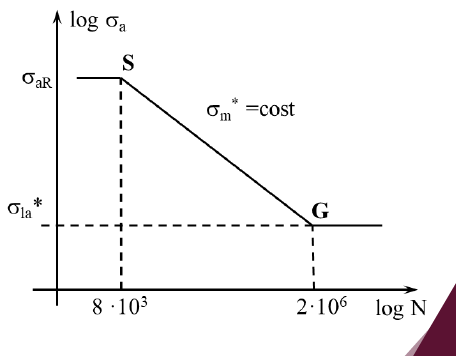
\includegraphics[width=0.2\linewidth]{immagini/screenshot021}
				\label{fig:screenshot021}
			\end{figure}			
			
			Ad esempio si identificano per un $ C40 $ dei valori di $ 710Mpa $ a rottura e $ 280Mpa $  di semiampiezza. 
			
			\begin{figure}[H]
				\centering
				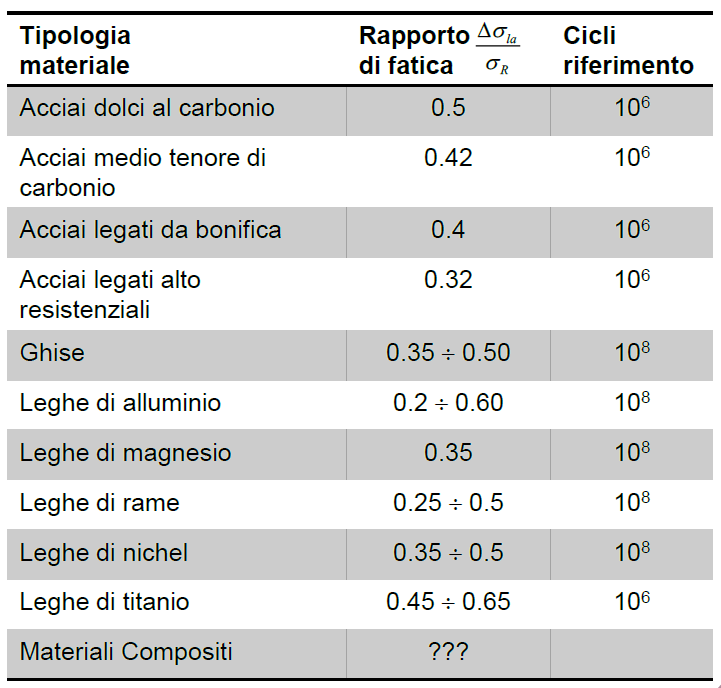
\includegraphics[width=0.3\linewidth]{immagini/screenshot022}
				\label{fig:screenshot022}
			\end{figure}
			
			In funzione poi della composizione dell'acciaio varietà il rapporto fra il limite di fatica e limite a rottura. Indicativamente per acciai legati in assenza  di una prova specifica di fatica si può prendere in prima approssimazione un rapporto compreso tra$  0.3 \div 0.5 $. Se $ 0.5 $ è un valore indicato per quelli al carbonio, acciai legati arrivano a $ 0.32 $, ma perché il legame con altri componenti riduce la durata a fatica? 
			
			Ad esempio i costosi acciai alto resistenziali che hanno altissimi valori di resistenza presentano però un rapporto di fatica basso, in generale materiali staticamente molto resistenti hanno, proporzionalmente, resistenza a fatica più bassa, il materiale alto resistenziale è un materiale che essendo più duro e nettamente più sensibile all'intaglio, e quindi al meccanismo di propagazione della cricca.
			
			Laddove poi nel materiale non c'è più ferro i rapporti di fatica divengono molto dispersi, il $10^6$ di limite diviene convenzionalmente $10^8$, non essendoci più un ginocchio nella curva, il problema va approcciato in modo statistico. \newline			
			
			\textbf{\Large Effetto della finitura superficiale e delle tensioni residue} \newline
			 Ogni valle tra due creste della rugosità del materiale è un potenziale innesco, minori sono queste valli, minori sono le probabilità di innesco.
			 
			 Un pezzo grezzo preso dalla fonderia è molto più probabile che faccia partire una cricca di fatica rispetto ad un materiale lavorato, rettificato e lucidato. Le stesse lavorazioni che portano alla rettifica della rugosità però sono lavorazioni meccaniche che interferiscono  con gli strati superficiale del materiale, ad esempio un trattamento superficiale di \textit{pallinatura}, che consister nel bombardamento del pezzo con palline d'acciaio duro, genera tensioni residue ma a quale scopo? Si creano infatti delle condizioni di stato tensionale residuo che vanno a contrastare un eventuale trazione, in più al tempo stesso si migliora la finitura superficiale, si ottiene così uno stato tensionale effettivo localmente più basso rispetto al picco, questo tipo di lavorazione tuttavia influenza uno spessore molto piccolo di materiale e genera anche una leggera trazione sottopelle, la superficie va in compressione e sottopelle va in trazione. 
			 
			 Altre \textbf{lavorazioni tecnologiche} includono la \textit{rullatura}
			 \begin{itemize}
			 	\item Rulli e dischi variamente sagomati
			 	\item Migliore finitura superficiale
			 	\item Profondità fino a circa 2 mm
			 	\item Pezzi assialsimmetrici (raccordi)
			 \end{itemize}
		 	 la \textit{sabbiatura}, utilizzata per la pulizia dei getti, la \textit{rettifica} e la \textit{lucidatura} che portano si a miglioramento superficiale ma indicono possibili tensioni di trazione, infine si fanno menzione delle \textit{macchine utensili} che lavorano per asportazione di truciolo, il taglio di queste induce però tensioni residue di trazione.\newline 
		 	 
			 Ciascuna di queste lavorazioni ha un impatto sulla durata, un diagramma come questo
			 
			 \begin{figure}[H]
			 	\centering
			 	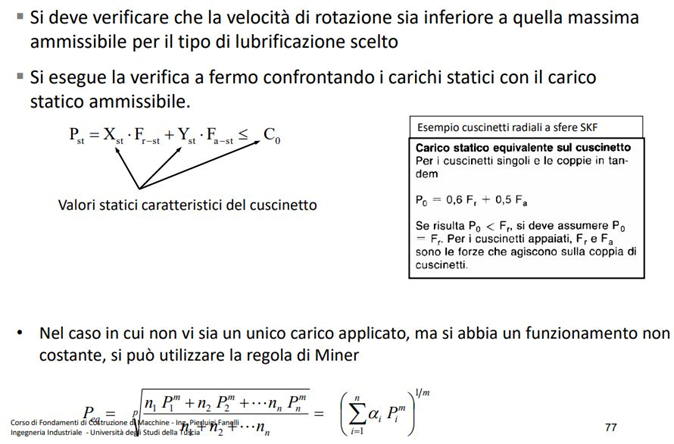
\includegraphics[width=0.5\linewidth]{immagini/screenshot023}
			 	\label{fig:screenshot023}
			 \end{figure}
			 
			Introduce un coefficiente correttivo della durata del pezzo, ma cosa corregge? Le condizioni standard.
			
		    Si parte cioè dal limite a fatica del provino (non del materiale) in condizioni standard, per cui se ce ne se discosta sarà necessario correggerlo.  
		    Il valore unitario, standard, si ha per un pezzo lucidato a specchio.
		    
		    In questo caso l'andamento è plottato in funzione della durezza anziché del limite di rottura,d'altro canto vale lo stesso dire che tanto più è duro o resistente staticamente il componente, tanto più si riduce il limite di fatica. 
		    
		    Per un pezzo laminato a caldo, se ha una resistenza bassa ed è dolce, non duro, ha un fattore correttivo pari allo $0.7$, al $ 70\% $ della condizione lucidata, se il pezzo è molto resistente o ha una durezza superficiale molto elevata si può arrivare anche a un fattore di riduzione pari al $ 30\% $ rispetto al provino standard. 
		    
		    Per questo le indicazioni di rugosità sono importanti nel disegno tecnico, il pezzo infatti lo si andrà a lucidare dove si avrà o un particolare montaggio con possibili strisciamenti, oppure dove localmente dovrà avere alta resistenza a fatica. \newline
			 
			Influenzano poi la durata a fatica di un componente i \textbf{trattamenti termici}. 
			
			Ad esempio la tempra si utilizza quando negli acciai si vuole un passaggio a martensite, in questo modo andando a modificare la struttura cristallina e aumentando il volume della stessa si dà vita ad una compressione residua che indurisce il componente è è in più favorevole alla durata a fatica dello stesso. 
			
			Altri trattamenti termici noti sono la carbocementazione e la nitrurazione, quest'ultimo in particolare è un tipo di trattamento termico che ha un limitato impatto sulla fatica al contrario dell'impatto che ha sulla resistenza ad usura. \newline 
			
			Un altro aspetto importante da considerare è il \textbf{rivestimento} del materiale, accade spesso infatti che un componente venga rivestito con dei metalli, ad esempio un rivestimento duro sarà in grado di rispondere meglio alle esigenze di contatto e quindi ridurre l'usura e aumentare la vita del componente, ma proprio perché è duro è un materiale molto più sensibile ad una cricca, ad un danneggiamento, se malauguratamente la placcatura dovesse criccasi questa cricca possiederà una concentrazione di tensione tale da portare il materiale sottostante ad un innesco estremamente pericoloso.
			
			 Finché si degrada il materiale superiore che ha o esigenze estetiche, o anti-usura, o di protezione alla corrosione, ma non ha assolutamente responsabilità strutturali, non è un gran problema; ma se questo incomincia a criccarsi e questa cricca arriva al materiale sottostante, venendosi a creare una fortissima concentrazione di tensioni mette in pericolo la resistenza strutturale dell'interno componente. \newline
			 
			 \textbf{\Large Effetto scala, effetto delle dimensioni} \newline
			 Un componente più grande dura meno rispetto ad uno più piccolo principalmente per due motivi. Il promo è prettamente statistico, siccome la superficie è più grande c'è molta più probabilità che ci siano difetti: dato che la fatica dipende dalla presenza di difetti nel materiale, un pezzo più grande ha più probabilità di avere un difetto.
			 
			 L'altro è legato sopratutto, per le sollecitazioni di flessione, al gradiente di tensione.
			 
			 \begin{figure}[H]
			 	\centering
			 	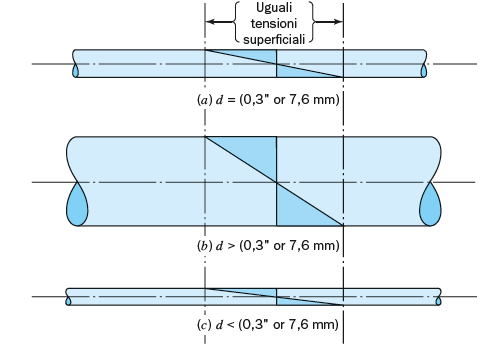
\includegraphics[width=0.5\linewidth]{immagini/screenshot024}
			 	\label{fig:screenshot024}
			 \end{figure}
			 
			 In presenza di un piccolo danneggiamento sulla superficie in un pezzo minuto, quando la cricca entra di $ 1mm $ nel pezzo, trova sotto di se una tensione che sta variando linearmente con lo spessore - o col raggio - che è già scalata di $1/3$: l'apice della cricca si trova ad uno stato tensionale molto più ridotto e progredisce molto più lentamente.
			 
			 Trovandosi invece su un pezzo più grande, essendo il gradiente molto più basso, a parità di tensione massima l'andamento a farfalla ha una pendenza molto diversa, è molto meno ripida: la cricca che di $ 1mm $ si trova ancora ad uno stato tensionale molto importante.
			 
			 Le dimensioni del pezzo hanno notevole impatto sulla durata a fatica \newline
			 
			 \textbf{\Large Corrosione} \newline 
			 Questa altera irrimediabilmente la superficie esterna, un elemento corroso porta ad una rugosità superficiale molto elevata. \newpage
			 
			 \textbf{\Large Effetto di forma, fattore effettivo di intaglio} \newline
			 In fatica la variazione di forma ha un impatto anche sui materiali duttili.
			\begin{figure}[H]
				\centering
				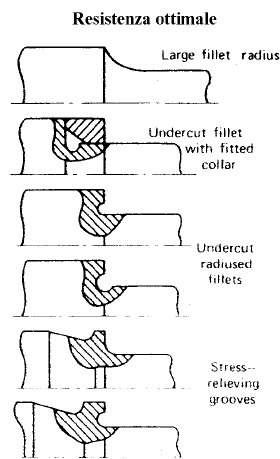
\includegraphics[width=0.5\linewidth]{immagini/screenshot025}
				\label{fig:screenshot025}
			\end{figure}
			
			Il coefficiente di forma o effettivo di tensione è definito come il rapporto tra il limite di fatica del provino senza intaglio e quello con l'intaglio.
			\[K_f = \dfrac{\text{limite di fatica SENZA intaglio}}{\text{limite di fatica CON intaglio}}\]
			Per materiali fragili si può utilizzare il $K_t$ anche per fatica, per i materiali duttili al contrario va determinato il $K_f$.
			
			 Questo $K_f$ è compreso tra l'unità e il $K_t$:
			 \[1<K_f<K_t\]
			 Non si può comunque andare oltre il  $K_t$ teorico di concentrazione di tensione.
			 Come si quantifica il  $K_f$? Tale fattore nella sua formulazione più utilizzata è funzione del  $K_t$ teorico e di un parametro $ q $, fattore di sensibilità all'intaglio del materiale
			 \[K_f = q(K_t-1) + 1 \hspace{1cm} q = \dfrac{K_f-1}{K_t-1}\] 
			 Perciò in funzione del tipo di materiale si può avere una diversa sensibilità all'intaglio, tale fattore essendo compreso tra 0 ed 1 indica con il valore nullo nessuna sensibilità all'intaglio mentre con valute unitario una sensibilità all'intaglio massima. Un acciaio alto resistenziale ha ad esempio una $ q $ prossima all'unità. \newline
			 
			 Nel grafico sottostante si può vedere la combinazione tra la sensibilità all'intaglio $ q $ e i livelli di sollecitazione limite a rottura, le varie curve rappresentano i valori di carico limite.
			 
			 \begin{figure}[H]
			 	\centering
			 	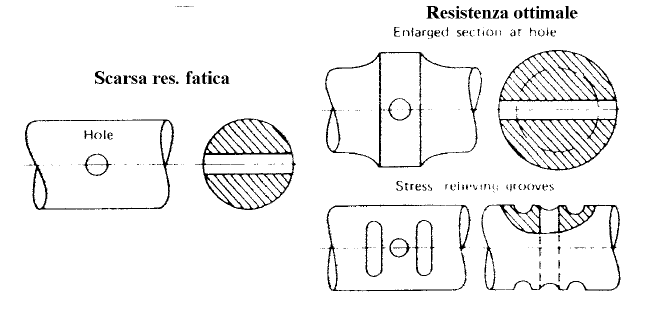
\includegraphics[width=0.5\linewidth]{immagini/screenshot026}
			 	\label{fig:screenshot026}
			 \end{figure}			 
			 
			   $ q $ dipende dalla geometria dall'intaglio e varia con la temperatura, all'aumentare di questa $ q $ diminuisce  e viceversa.
			   
			   Ricordi l'aneddoto per cui le navi da trasporto \textit{Liberty Ship} in acqua gelida cedevano a fatica? Quello stesso materiale a basse temperature aumentava la sua $ q $, la sua sensibilità all'intaglio e quindi un piccolo difetto portava ad una maggiore probabilità di rottura. \newline
			   
			 Come impatta la $K_f$ sulla curva di Wöhler?
			 
			 Sposta il ginocchio della cura di Wöhler, il provino con l'intaglio avrà un ginocchio spostato più  in  basso rispetto al provino standard, sempre posto allo stesso numero di cicli. 
			 
			 \begin{figure}[H]
			 	\centering
			 	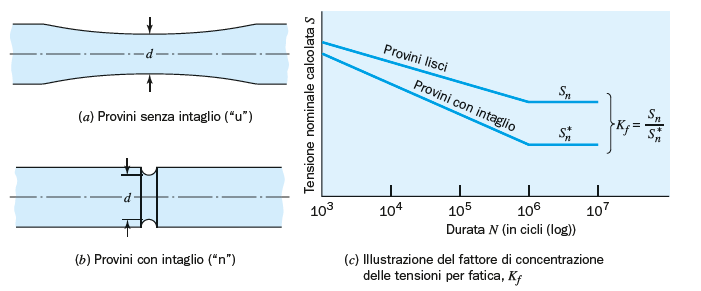
\includegraphics[width=0.5\linewidth]{immagini/screenshot027}
			 	\label{fig:screenshot027}
			 \end{figure}			 
			 
			 Il rapporto tra i ginocchi rappresenta proprio la $K_f$. \newline
			 
			 Esistono tante relazioni che determinano la $ q $, questa subito riportata è quella di Neuber ed è adatta per gli acciai.
			 \[q = 1+\dfrac{\pi}{\pi-\alpha}\cdot\sqrt{r_n\over r}\]
			 Dove $\alpha$ è l’angolo dell’intaglio al fondo gola ed
			 \[r = 0.02\left(1-{R\over S}\right)^3\left(1-{0.05\over d}\right)\]
			 Essendo $ d $ la dimensione minima del provino; $ R $ ed $ S $ rispettivamente il carico di rottura e di snervamento del  materiale.\newline 
			 
			 Tra le relazioni per la determinazione del $K_f$ si menziona quella di Petersen nella quale introduce il gradiente di tensione.
			 \[K_f = 1+ \dfrac{K_t}{\left[ik + \sqrt{K_1\chi}\right]}\]
			 dove $\chi$ è il gradiente delle tensioni; $ ik $ è funzione della duttilità del materiale e
			 $ K_1 $ dipende dalla durezza superficiale secondo la relazione \(K_1 = ({40\over HV})^2\)
			 
			 \vspace{1cm}			   
			 Si analizzeranno adesso i parametri esterni, le modalità di lavoro del componente, il modo in cui viene utilizzato il componente, le caratteristiche di carico e ambientali che lo circondano. \newpage
			 \vspace{1cm}
			 
			 \textbf{\Large Tipo di sollecitazione} \newline
			 NB: si sta considerando la tipologia di sollecitazione, non le modalità del carico. 
			 
			 Nelle applicazioni meccaniche si avrà a che fare principalmente con flessione, trazione e torsione  cicliche, meno frequentemente si avrà una condizione ciclica sul taglio. \newline 
			 
			 La flessione in condizioni di sollecitazione costante nel tempo si traduce, in casi di elemento rotante, in uno stato tensionale variabile nel tempo. Ad esempio nel caso di un albero di trasmissione ci si troverà di fronte ad una condizione di carico caratterizzata da una flessione rotante ma una torsione costante nel tempo, se poi non c'è neanche variazione del rapporto di trasmissione si avrà una torsione costante.
			 
			 In funzione della tipologia di sollecitazione ciclica e quindi delle tensioni cicliche derivanti si avrà una variazione della durata a fatica del componente. \newline
			 
			 Se si riporta su un diagramma di Wöhler le diverse sollecitazioni, ovvero i dati sperimentali dello stesso provino soggetto a sollecitazioni differenti le curve si modificano in modo considerevole. \newline
			 
			 Si nota infatti come la flessione è quella sollecitazione che garantisce una durata maggiore, mentre scendendo si incontrano trazione-compressione pure ed infine torsione. 
			 
			 Le curve di Wöhler relative alla tipologia di sollecitazione vengono convenzionalmente modificate da coefficienti che spostano sul piano i due punti d'interesse: quello a $10^3$ cicli e il ginocchio a $10^6$ cicli, mentre il valore della tensione è invece un valore che deve essere fissato.
			 
			 In realtà il punto che serve a tracciare la curva è soltanto il ginocchio, infatti solitamente il punto a $10^3$ cicli è dato dal valore di rottura in condizioni standard statiche (flessione). Alcuni codici consigliano di prendere lo $ 0.9 $ del valore a rottura, infatti in funzione del codice scelto (UNI7670, EuroCodice) quel punto è fissato in funzione del carico di rottura, per cui non c'è alcun bisogno di eseguire prove sul materiale, per identificare quel punto bastano i valori di targa statici; il test servirà quindi a caratterizzare il ginocchio ovvero il limite di fatica $ S_n $ o $\sigma_{la}$, equivalentemente per acciai questo valore lo si può perdere pari al $ 50\% $ del carico ultimo a flessione. 
			 
\begin{figure}[H]
	\centering
	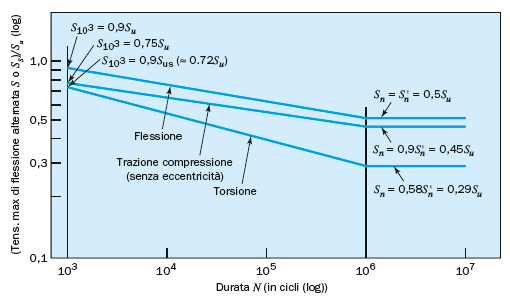
\includegraphics[width=0.5\linewidth]{immagini/screenshot028}
	\label{fig:screenshot028}
\end{figure}			 
			 
			 Per cui il limite di sinistra, quello per la fatica oligociclica, viene ridotto al $ 90\% $ per la flessione, al $ 75\% $ per la trazione e al $ 90\% $ percento della $\tau$  ammissibile a torsione, oppure utilizzando Von Mises al $ 90\% $ del carico utile diviso $\sqrt{3}$, ugualmente anche per il ginocchio, per il limite di fatica, lo si usa ridurre attraverso l'utilizzo di un fattore.
			 
			 Se infatti si riportano questi fattori su un diagramma $ \sigma_1\sigma_2 $ di Von Mises in condizioni piane, i limiti imposti non sono altro che dei coefficienti che traducono lo stato tensionale in valori equivalenti, quei fattori correttivi sono infatti i fattori utilizzati per ricavare le tensioni equivalenti in condizioni statiche con Von Mises il fattore $ 0.58 $ trovato nella trasformazione della tensione è il termine che permette di stare all'interno dell'ellisse nel quarto quadrante nel passaggio da $\tau_{amm}$ a $\sigma_{amm}$. \newline 
			 
			 Nei materiali duttili la resistenza a fatica in caso di sollecitazioni di torsione alternata risulta circa pari al $ 58\% $ di
			 quella a flessione alternata (in accordo con la formulazione di Von Mises).
			 Il
			 limite ultimo statico a taglio è circa $ 80\% $ di quello a trazione per gli acciai ($ 70\% $ per i materiali duttili in genere)
			 
			 			 \begin{figure}[H]
			 	\centering
			 	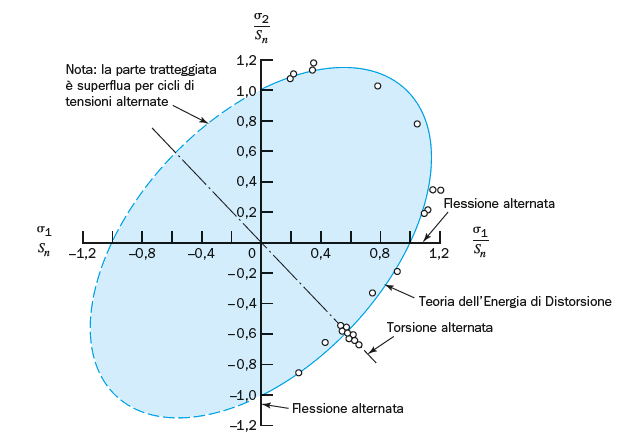
\includegraphics[width=0.5\linewidth]{immagini/screenshot029}
			 	\label{fig:screenshot029}
			 \end{figure}
			 			 
			 \textbf{\Large Temperatura}\newline
			 Nel caso dell'influenza della temperatura il discorso è simile a quello effettuato in condizioni statiche, per cui una temperatura che aumenta riduce la sensibilità del materiale all'intaglio e rende il materiale più duttile e meno fragile aumentando la durata a fatica, mentre una temperatura più bassa porta ad un comportamento fragile con una resistenza a fatica che diminuisce. 
			 
			 Oltre alla sensibilità all'intaglio però, nel caso di aumento di temperatura si evidenzia purtroppo un doppio trend, infatti quando si arriva a temperature che si avvicinano anche solo alla metà di quelle di fusione $0.4T_{fus}$, si innescano fenomeni legati allo scorrimento viscoso del materiale: si evidenzia infatti in questo una dipendenza delle deformazioni dal tempo oltre che dal carico. 
			 
			 In questo modo l'applicazione di un carico costante porta a variazioni di deformazione nel tempo e l'applicazione di un carico variabile nel tempo porta a deformazioni ancor più variabili nel tempo. Ad esempio un carico applicato a $t_0$ genera una deformazione legata al carico $t_0$ che cresce nel tempo, per cui quando si andrà ad applicare un carico $t_1$ si troverà un oggetto ancora deformato per il carico $t_0$. \newline
			 
			 Le ipotesi fatte all'inizio della trattazione della fatica prevedevano che questa era assimilabile ad una successione di condizioni statiche, tale ipotesi implica che applicando il carico si ottiene istantaneamente un effetto che si annulla rimuovendo il carico, la presenza di uno scorrimento viscoso invece invalida queste ipotesi: applicando il carico se ne vede l'effetto nel tempo e rimuovendo il carico si continua a vederne l'effetto, in questo modo quando poi si va nuovamente a riapplicare il carico si ritrova una condizione già deformata. \newline 
			 
			 Il range di temperature per le quali si ha un comportamento senza \textit{creep} viscoelastico è tra 0\degree C e 200\degree C. Per gli acciai di normale applicazione, all'interno di questo range sono garantite le condizioni standard di fatica. \newpage
			 
			\textbf{\Large Frequenza di applicazione del carico}\newline
			 L'ipotesi per cui la fatica è assimilabile ad una successione di carichi statici è vera solo se il carico ha una frequenza di applicazione piuttosto bassa; un'applicazione di carico più veloce e quindi a più alte frequenze implica che il materiale no sia più in grado di rispondere in tempo reale alle sollecitazioni dando vita ad uno sfasamento tra causa ed effetto, ovvero tra forza e risposta, che porta alle amplificazioni dinamiche. \newline 
			 
			 L'ipotesi aggiuntiva che si fa dunque per evitare questo tipo di amplificazione è quella per cui la frequenza di applicazione del carico non superi gli $80$ Hz, infatti sotto questa soglia e tanto diviene più bassa la frequenza di applicazione del carico, tanto più acquisisce validità l'ipotesi di partenza. Di contro all'aumentare della frequenza si crea un effetto di isteresi (comportamento viscoelastico) della risposta del materiale con presenza di surriscaldamenti con variazione locale di temperatura, sopra 150 Hz c'è addirittura l'instaurazione di una dinamicità della risposta: si ha una sovrapposizione dinamica degli effetti, con dati irregolari e il paradossale aumento di resistenza a fatica, le tensioni interne del materiale seguono in ritardo la sollecitazione esterna. \newline
			 
			 La dipendenza dalla frequenza è un elemento da tenere in considerazione durante le prove di laboratorio. Naturalmente occupare una macchina per tanto tempo è un costo importante, per cui si cerca di aumentare il più possibile la frequenza di applicazione facendo attenzione che questa non influenzi il risultato finale. 
			 
			 Perciò per ottenere un risultato il prima possibile si cerca di aumentare la frequenza di sollecitazione mitigando gli effetti di surriscaldamento e isteresi raffreddando il componente, facendo tuttavia sempre attenzione  che abbassare la temperatura porta a variazioni del limite di fatica, si sta andato ad aumentare la sensibilità all'intaglio del componente. \newline 
			 
			\textbf{\Large Effetto del ciclo di carico}\newline
			\begin{figure}[H]
				\centering
				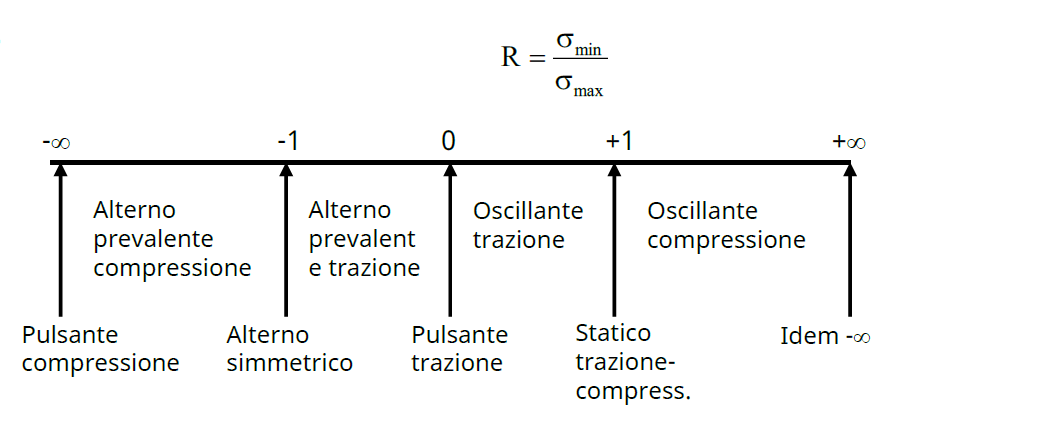
\includegraphics[width=0.5\linewidth]{immagini/screenshot030}
				\label{fig:screenshot030}
			\end{figure}			
			 
			 Questa tabella riporta i valori di riferimento per rapporto di ciclo $ R = {\sigma_{\min}\over\sigma_{\max}} $ in funzione della tipologia dello spettro di carico. \newline
			 
			 $ R=-1 $ è tipico dell'alterno simmetrica, ovvero della flessione rotante dove $ \max=\min $ in modulo con media nulla. 
			 
			 Le pulsazioni di trazione e compressione si hanno per un rapporto $ R=0 $ per cui la $\min=0$ mentre $\max>0$ di trazione.
			 
			 $R=-\infty$ per pulsazioni di compressione, la $\min<0$ mentre $\max=0$ e ugualmente varrà per $R=+\infty$.
			 
			 La $ R=1 $ è il caso di condizione statica di trazione o di compressione, non si è in grado di distinguerla perché il rapporto dà sempre il valore unitario. \newpage
			 
			 I valori intermedi tra $ \left[-\infty; -1\right] $ sono quelli che danno le famiglie alterno simmetriche a prevalente compressione, in pratica si ha in questo caso:
			  
			 \begin{figure}[H]
			 	\centering
			 	\begin{tikzpicture}[scale = 0.75]
			 	\begin{axis}[
			 		%xlabel=$x$,
			 		%ylabel=$\sin(x)$,
			 		domain=0:6*pi,  
			 		samples=200,
			 		axis lines=middle,
			 		%grid=both,
			 		xtick={}, ytick={}, 
			 		xticklabels={}, yticklabels={},
			 		]
			 		\addplot[blue, thick] {sin(deg(x))- 0.5};
			 	\end{axis}
			 \end{tikzpicture}
			 \end{figure}
			 
			 Per cui prevalente di compressione significa dire che la tensione minima ha un modulo molto più grande della tensione massima.
			 
			 Tra $ \left[-1; 0\right] $ si ha
			  
			 			 \begin{figure}[H]
			 	\centering
			 	\begin{tikzpicture}[scale = 0.75]
			 		\begin{axis}[
			 			%xlabel=$x$,
			 			%ylabel=$\sin(x)$,
			 			domain=0:6*pi,  
			 			samples=200,
			 			axis lines=middle,
			 			%grid=both,
			 			xtick={}, ytick={}, 
			 			xticklabels={}, yticklabels={},
			 			]
			 			\addplot[blue, thick] {sin(deg(x))+ 0.5};
			 		\end{axis}
			 	\end{tikzpicture}
			 \end{figure}
			 
			 Tra $ \left[0; 1\right] $ sono entrambe positive
			  
			 			 			 \begin{figure}[H]
			 	\centering
			 	\begin{tikzpicture}[scale = 0.75]
			 		\begin{axis}[
			 			%xlabel=$x$,
			 			%ylabel=$\sin(x)$,
			 			domain=0:6*pi,  
			 			samples=200,
			 			axis lines=middle,
			 			%grid=both,
			 			xtick={}, ytick={}, 
			 			xticklabels={}, yticklabels={},
			 			]
			 			\addplot[blue, thick] {sin(deg(x))+ 2.5};
			 		\end{axis}
			 	\end{tikzpicture}
			 \end{figure}
			 
			 Tra $ \left[1; +\infty\right] $ invece
			 
			 			 			 			 \begin{figure}[H]
			 	\centering
			 	\begin{tikzpicture}[scale = 0.75]
			 		\begin{axis}[
			 			%xlabel=$x$,
			 			%ylabel=$\sin(x)$,
			 			domain=0:6*pi,  
			 			samples=200,
			 			axis lines=middle,
			 			%grid=both,
			 			xtick={}, ytick={}, 
			 			xticklabels={}, yticklabels={},
			 			]
			 			\addplot[blue, thick] {sin(deg(x))- 2.5};
			 		\end{axis}
			 	\end{tikzpicture}
			 \end{figure}
			 
			 
			 A parità di semiampiezza di sollecitazione è evidente perciò che la durata a fatica sia completamente diversa in questi 4 casi, proprio per il meccanismo di apertura della cricca che porta al cedimento del componente, per cui una $\sigma_m$ di trazione, a parità di semiampiezza, è una condizione più critica, mentre naturalmente, a parità di semiampiezza una $\sigma_m$ di compressione è molo favorevole alla durata a fatica, perché tende a tenere chiusa la cricca. \newline
			 
			 Se si lavora invece a parità di tensione massima $\sigma_{\max} = \sigma_m + \sigma_{la}$, facendo variare la tensione media è evidente che si debba avere un spettro di carico con una semiampiezza più piccola, per cui se si lavora con una tensione massima di progetto che è necessario mantenere, ad esempio magari non si può andare oltre lo snervamento, allora si dovrà valutare uno spettro di carico che potrà avere differenti tensioni medie ma un'ampiezza minore dello snervamento. Questa condizione vuol dire legare la semiampiezza al valore medio, quindi una tensione media di trazione che si è appena detto essere sfavorevole, ragionando per tensioni medie, in realtà è accompagnata da una semiampiezza molto piccola. \newline
			 
			 Quella che si valuta sperimentalmente a parità di carico massimo è la condizione peggiore, ovvero quella che prevede una $\sigma_m=0$, e sforzo puramente alternato. Infatti partendo da questa condizione e aumentando
			 la tensione media, sia nel verso della compressione e sia nel verso della trazione, la resistenza aumenta
			 (ragionando sempre in termini si stessa tensione massima).
			 
			 Quale delle tre, immaginando semiampiezze uguali, è la condizione peggiore?
			 
			 \begin{figure}[H]
			 	\centering
			 	\begin{tikzpicture}
			 	\begin{axis}[
			 		xlabel=$x$,
			 		ylabel=$y$,
			 		domain=0:6*pi,
			 		samples=200,
			 		axis lines=middle,
			 		%grid=both,
			 		axis background/.style={fill=none},
			 		xtick={}, ytick={},
			 		xticklabels={}, yticklabels={},
			 		]
			 		
			 		% Sinusoide totalmente positiva
			 		\addplot[blue, thick] {sin(deg(x)) + 1} node[above, pos=0.7] {I};
			 		
			 		% Sinusoide alternata positiva-negativa
			 		\addplot[red, thick] {sin(deg(x))} node[above, pos=0.5] {II};
			 		
			 		% Sinusoide totalmente negativa
			 		\addplot[green!70!black, thick] {-sin(deg(x)) - 1} node[below, pos=0.7] {III};
			 		
			 	\end{axis}
			 \end{tikzpicture}
			 \end{figure}
			 
			 La prima, quella che ha una sigma media di trazione. \newline
			 
			 Lavorando a parità d tensione massima 
			 
			 	\begin{figure}[H]
			 		\centering
			 		\begin{tikzpicture}[scale = 0.75]
			 	\begin{axis}[
			 		%xlabel=$x$,
			 		%ylabel=$y$,
			 		domain=0:6*pi,
			 		samples=200,
			 		axis lines=middle,
			 		%grid=both,
			 		xtick={}, ytick={},
			 		xticklabels={}, yticklabels={},
			 		ymin=-2,  % Imposta il limite inferiore dell'asse y
			 		ymax=3,   % Imposta il limite superiore dell'asse y
			 		]
			 		
			 		% Sinusoide positiva
			 		\addplot[blue, thick] {sin(deg(x)) + 1} node[above, pos=0.5] {I};
			 		
			 		% Sinusoide alternata
			 		\addplot[red, thick] {2*sin(deg(x/2))} node[above, pos=0.8] {II};
			 		
			 		% Sinusoide alternata ampia
			 		\addplot[green!70!black, thick] {2*sin(deg(x/4))} node[below, pos=0.2] {III};
			 		
			 		% Linea orizzontale a y=2
			 		\draw[dashed, black] (axis cs: 0,2) -- (axis cs: 6*pi,2);
			 	\end{axis}		
			 \end{tikzpicture} 
			 	\end{figure}
			 
			 La peggiore è la seconda, quella con tensione media nulla, è vero che la prima ha una tensione molto più alta di trazione però è anche vero che le si associa una semiampiezza molto piccola.\newline 
			 
			 In figura, qualitativamente, le differenti configurazioni di carico  
			 
			 \begin{figure}[H]
			 	\centering
			 	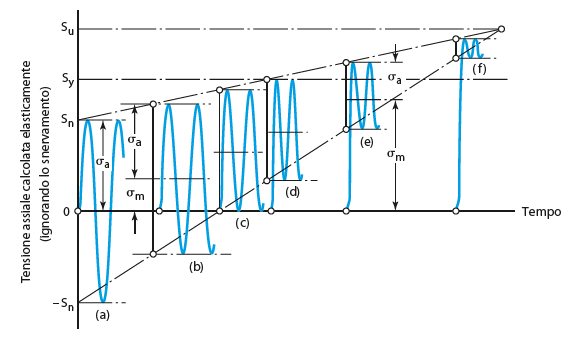
\includegraphics[width=0.5\linewidth]{immagini/screenshot031}
			 	\label{fig:screenshot031}
			 \end{figure}
			 
			 In questo caso si sta lavorando considerando la condizione statica di rottura e una condizione perfettamente alterno simmetrica con un limite sullo snervamento, questo può essere visto quindi come un campionamento di condizioni critiche tra una condizione alterno simmetrica e una condizione statica, quindi per avere parità di condizione all'aumentare del carico medio di trazione si deve ridurre la semiampiezza. \newline
			 
			 \textbf{\Large Storia del carico}\newline
			 Estremamente importante è l'elemento più aleatorio che si ha nel fenomeno di fatica, influenza notevolmente le previsioni e purtroppo ad oggi non vi è ancora una modellizzazione sufficientemente approfondita che permetta di avere una predizione matematica - sia pur affetta dal problema statistico - soddisfacente, ci si deve piuttosto basare su valori di riferimento sperimentali. \newline
			 
			 Quando si è visto che i cicli di carico sono caratterizzati da una tensione media e da una semiampiezza, si è detto che la condizione di studio è quella   di un singolo ciclo di applicazione del carico variabile sinusoidalmente con parametri costanti nel tempo. Si è però poi detto che il caso reale presenta però un andamento nel tempo molto più complesso, si è così individuata con metodi approssimati una serie di cicli equivalenti che messi insieme danno lo stesso danneggiamento del ciclo reale. Questo vuol dire che gli stessi cicli equivalenti messi in successione, uno dopo l'altro, dovranno dare la stessa vita a fatica di un ciclo reale.
			 
			 Al tempo stesso si può manifestare in realtà anche una situazione che preveda una successione temporale di cicli differenti.
			 
			 Perciò sia nella trasformazione di un caso reale in una successione di casi equivalenti che nell'applicazione in successione reale di casi semplici, si ottiene un effetto di fatica dovuto a cicli sinusoidali differenti sovrapposti l'uno sull'altro. Purtroppo in fatica non esiste la semplificazione data dalla
			 sovrapposizione lineare degli effetti come in un problema elastico, ma il tutto viene trattato secondo un modello di danno che il singolo ciclo causa sul componente.\newline
			 
			 La teoria di
			 Palmgren-Miner si basa sull’ipotesi dell’accumulo lineare degli effetti della fatica, definendo il danneggiamento come la combinazione dei danni fatti da ciascun singolo ciclo di carico pesato su un limite che si avrebbe applicandolo separatamente.\newpage
			 
			 Si immagini di avere $\sigma_1, \sigma_2$ semiampiezze di sollecitazioni a cui sono associati un certo numero di cicli a rottura per fatica $ N_1, N_2 $ questo vuol dire che se si prende la curva caratteristica doppio logaritmica di Wöhler a $ \sigma_1 $ corrisponde $ N_1 $ e a $ \sigma_2 $ corrisponde $ N_2 $.
			 		
\begin{figure}[H]
	\centering
				 \begin{tikzpicture}[>=latex, scale = 0.75]
			 	%%%	Help Lines
%			 	\draw [thin, help lines] (0,0) grid (10,10);
%			 	\foreach \x in {0,...,10}
%			 	\draw (\x cm,1pt) -- (\x cm,-1pt) node[anchor=north] {$\x$};
%			 	\foreach \y in {0,...,10}
%			 	\draw (1pt,\y cm) -- (-1pt,\y cm) node[anchor=east] {$\y$};
			 	%%%	Disegno	
			 	\draw[->] (0,0) -- (0,5) node [pos = 1, above] {$\sigma$};
			 	\draw[->]  (0,0) -- (10,0) node [pos = 1, right] {$N$};
			 	\draw (1,5) .. controls (2,3) and
			 	(6,1) .. (10,1);
			 	
			 	\draw[blue] (0, 3) -- (3, 3) node [pos=0, left] {$\sigma_1$};
			 	\draw[blue] (3, 3) -- (3, 0) node [pos=1, below] {$N_1$};
			 	
			 	\draw[green!70!black] (0, 2) -- (5, 2) node [pos=0, left] {$\sigma_2$};
			 	\draw[green!70!black] (5, 2) -- (5, 0) node [pos=1, below] {$N_2$};
			 	
			 \end{tikzpicture}
\end{figure}
			 
			 $ N_1, N_2 $ sono il numero di cicli limite che quel componente potrebbe sopportare applicando quella determinata semiampiezza, $ n $  è invece il numero di cicli effettivamente applicato. Ad esempio dire che se a 100 MPa di semiampiezza di sollecitazione corrispondono $ N=10^5 $ cicli come numero massimo di cicli di applicazione del carico, si può equivalentemente applicarne un numero inferiore $ n $ senza avere la rottura a fatica, il danno che si introduce sul pezzo applicando un numero inferiore è proporzionale al rapporto tra queste grandezze, quindi se $\sigma_1$ = 100 MPa al quale corrispondo magari $10^5$ cicli di applicazione come limite ultimo: se sono stati applicati in realtà $10^4$ cicli ho esaurito il 10\% della durata a fatica del componente, contribuendo ad un danno dello 0,1. 
			 
			 Se successivamente di applica un carico $\sigma_2$=50 MPa il limite magari diventa $5\dot10^5$ se questi 50 MPa li ho applicati per $10^5$ cicli, va fatto $D = \dfrac{10^5}{\dot10^5}$ pari a 0,2: il danno accumulato sommando tutti i cicli diviene 0,1+0,2=0,3. \newline 
			 
			 Quando ci si ferma?
			 			 
			 Palmgren-Miner nella loro prima versione della teoria evidenziavano un limite pari ad 1 se vengono sommati due cicli, per cui, finché la somma del danno non arrivava all'unità, non si vedevano problemi; va da se che tale limite valeva uno anche per singolo ciclo, ovvero quando il numero di cicli$ n=N$: se c'è solo un ciclo di applicazione, ci si ferma a quel valore trovato.
			 
			 Per individuare $N_1$ sul diagramma di Wöhler ci si deve ricordare che la curva corrisponde a una determinata probabilità di sopravvivenza, nel diagramma classico la curva corrisponde al 90\% di probabilità che il provino sia ceduto. \newline 
			 
			 Per cui dire che il provino si rompe non appena viene applicato esattamente questo numero di cicli e quando il rapporto tra cicli $n/N$ è unitario, non è sempre vero, c'è una certa incertezza, una dispersione dei dati, motivo per cui la legge di Palmgren-Miner e poi la legge generalizzata di Miner - che poneva la sommatoria dei rapporti pari - non è sperimentalmente vera, è estremamente conservativa, tant'è che proprio sperimentalmente  la sommatoria dei danneggiamenti dovuti ai singoli cicli oscilla tra 0,7 e 2,0: perché? 
			 
			 Un po' per la dispersione statistica dei casi sperimentali: la dispersione rispetto al numero di cicli è estremamente più grande della dispersione rispetto al livello di carico, e quindi dato che nel danneggiamento entra elusivamente il numero di cicli, si ha una dispersione di valori notevole rispetto alle regole teoriche. 
			 
			 La legge di Palmgren-Miner è talvolta non cautelativa, soprattutto perché non considera la storia di carico, infatti a carichi crescenti (ovvero cicli a livelli di carico sempre più grandi), corrispondono valori più alti del danneggiamento limite $D_{lim} = \sum D_i = \sum \dfrac{n_i}{N_i}$. \newpage
			 
			 Si è già detto come applicando un carico di bassa intensità poco il componente si danneggia poco, al contrario alte intensità aprono cricche e portano a rottura. 
			 
			 Applicando perciò sin da subito un carico elevato, questo porta giocoforza all'innesco di cricche, quando poi si applicano carichi decrescenti - ora che la cricca è innescata -  anche questi contribuiranno al suo avanzamento: con una successione di carichi decrescenti si può arrivare a livelli di $D$ più bassi. 
			 
			 Sperimentalmente si è addirittura notato che occasionali (non ciclici) sopraccarichi di trazione (overloads) portano ad un miglioramento della vita del pezzo; questo fenomeno è legato al fatto che localmente alla cricca avviene la plasticizzazione della sezione che incrudisce e quindi ne si rallenta localmente l'avanzamento. \newline
			 
			 Purtroppo per il danneggiamento non c'è una legge analitica di riferimento che dia un valore limite consolidato, di cui ci si possa fidare ciecamente, per cui di volta in volta si dovrà considerare il modello di studio più adeguato: spesso si utilizza quello più conservativo per poter avere una stima "peggiorativa" del risultato di durata. \newline 
			  
			 Un'ulteriore argomento da trattare riguarda la rappresentazione dell'accumulo del danno. 
			 
			 Le condizioni che portano ad un accumulo del danno sono una successione di carichi variabile nel tempo che di solito vengono rappresentati come un terno di sollecitazioni attraverso un istogramma di carico o come una funzione continua data dalla una sommatoria dei cicli effettivi di applicazione.
			 \begin{figure}[H]
			 	\centering
			 	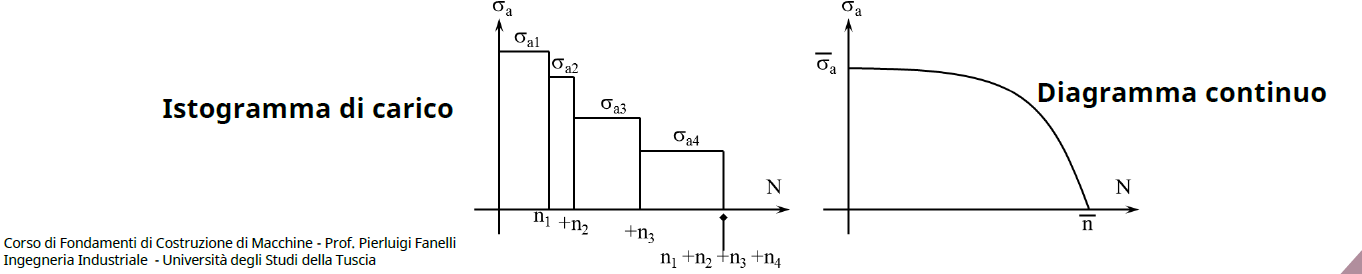
\includegraphics[width=\linewidth]{immagini/screenshot032}
			 	\label{fig:screenshot032}
			 \end{figure}		 
				Sull'istogramma si può porre la reale successione dei carichi come i cicli equivalenti ottenuti dalla regola del serbatoio. \newline
				
				Più spesso è utile utilizzare la legge di accumulo del danno per valutare un singolo ciclo equivalente: testato che la combinazione di questi cicli deve dare un danneggiamento - per semplicità - pari a 1 allora potrebbe essere comodo provare un solo spettro di carico caratterizzato da una certa semiampiezza e da un certo numero di applicazioni tale che dia lo stesso identico danneggiamento della sommatoria dei singoli cicli, e quindi lavorare con una sola semiampiezza, una sola $\sigma_m$ ed un solo numero limite di cicli applicati e applicabili. \newline
				
				Partendo poi dal presupposto che l'obiettivo è quello di ottenere lo stesso livello di danneggiamento, cioè che la sommatoria di $n/N$ sia il numero che posto, allora il ciclo equivalente dovrà avere lo stesso danneggiamento $n/n$, tuttavia ponendo $D=1$ si trovano infinite coppie $(n,N)$ che soddisfano quel rapporto, che giocoforza dovrà essere limitato.
				
				Si deve applicare il ciclo equivalente per un numero di applicazioni $n$ che poterà al danno dei cicli reali per il numero massimo di cicli che si potrebbero applicare in condizioni equivalenti.
				
				Questo ciclo equivalente appartiene comunque al diagramma di Wöhler, è un punto sulla curva, una condizione limite per quel materiale o specifico componente, per cui è in relazione a qualsiasi ciclo di carico applicato, quindi se si individua un altro punto sulla curva (NB: $\Delta\sigma$ è un altro modo per dire semiampiezza) al di sotto dei valori equivalenti, Si possono porre in relazione grazie alla seguente formula:
				\[\sigma^cN=\,\text{cost}\]				
				Di $n_{eq}$ e $\sigma_{eq}$ esistono infinite coppie arbitrarie che soddisfino questa relazione, allora posso decidere di scegliere arbitrariamente la $\sigma_{eq}$ e ricavare la $n_{eq}$ o viceversa. La condizione di criticità a fatica è una combinazione di carico e durata, c'è una variabile in più rispetto alla condizione critica statica, in condizioni statiche c'è criticità quando raggiungo il carico limite, in fatica la criticità è legata sia al carico che a quante volte lo applico: ho la stessa criticità se applico tante volte un carico basso o poche volte un cario alto.
				
				Fissando il carico ovvero, la $\sigma_{eq}$, il numero di cicli di applicazione di quel carico equivalente affinché si individui lo stesso danno del caso reale è dato da questa relazione:
				\[n_{eq} = \left(\sum \dfrac{n_i}{N_i}\right)\cdot N_{eq}\]
				Trovo così qual è il numero di applicazioni del carico che ho scelto arbitrariamente al fine di ottenere lo stesso danno del treno di cicli di carico reale. \newline 
				
				In alternativa, ed è solitamente il metodo più utilizzato, si fissa il numero di applicazioni equivalenti come la sommatoria delle applicazioni reali, si fa una sostituzione inversa e si ottiene il carico equivalente come:
				\[\Delta\sigma_{eq} = \sqrt[k]{\dfrac{n_1\Delta\sigma_1^k + n_2\Delta\sigma_2^k + \dots + n_t\sigma_t^k }{\sum_in_i}}\]		
				Ovvero la conversione da una successione di carichi ad un carico equivalente, col quale meglio si potranno visualizzare i carichi di fatica. \newline
				
				{\Large \textbf{Normativa}} \\								
				Tutti questi fattori che aumentano o diminuiscono la durata a fatica di un componente, si devono tradurre in numero. \newline
				
				Per la fatica non esiste sostanzialmente una normativa univoca e chiara che dica come scegliere dei coefficienti, nelle normative italiane non vi è una norma che tratta il calcolo a fatica dei componenti meccanici. L'unico codice che fa cenno in modo quantitativo al dimensionamento di alberi meccanici a fatica è la UNI 7670, anni '70 mai aggiornata, e fa riferimento al dimensionamento di organi di sollevamento. Al suo interno c'è una sezione che tratta la valutazione dell'accumulo del danno e la fatica sui componenti meccanici. 
				
				Un altro riferimento lo si ottiene grazie all'euro-codice sezione 3, che prevede una proceduta di calcolo a fatica ma si limita ad poche tipologie di componenti ed ha più interesse civile che meccanico-industriale. \newpage
								
				Un approccio intermedio, sufficiente a chiare ad aggiornato, si trova sullo JUVINALL o sullo CHINLEY. 
				
				Il primo prevede prevede l'introduzione di questi fattori di correzione. 
				\begin{figure}[H]
					\centering
					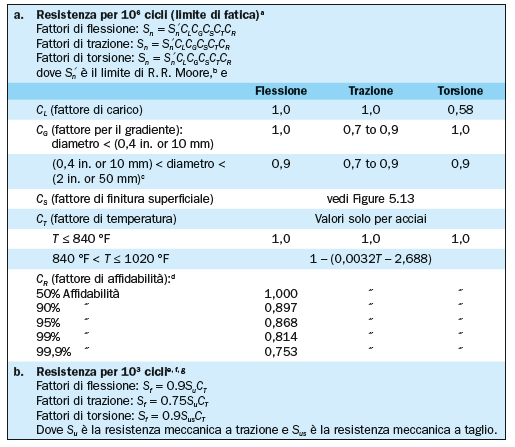
\includegraphics[width=0.7\linewidth]{immagini/screenshot033}
					\label{fig:screenshot033}
				\end{figure}
				\begin{figure}[H]
					\centering
					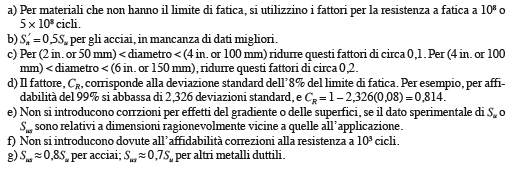
\includegraphics[width=0.5\linewidth]{immagini/screenshot034}
					\label{fig:screenshot034}
				\end{figure}
												
				La resistenza a $10^6$ cicli, cioè il limite di fatica, il valore da assegnare al ginocchio della curva di Wöhler viene preso considerando il valore di laboratorio $S_n'$.
				
				I successivi fattori correttivi assumono valori differenti in funzione della tipologia di sollecitazione.  
				
				\begin{itemize}
					\item A cosa sono dovuti i fattivi $C_L?$
				
				Da Von Mises è noto che la $\sigma_{eq}$ è data 
				\[\sigma_x^2 - \sigma_x\sigma_y + \sigma_y ^2+ t\tau^2_{xy}\] 
				Se si ha solo torsione rimane $\tau$ e la $\tau$ ammissibile di torsione dovrà essere il limite di fatica fratto radice cubica: è la conversione da $\sigma$ a $\tau$ di Von Mises. 
				
				\item $C_G$ è un fattore di gradiente, di dimensione: per un diametro del componente più grande mi aspetto che duri di meno, perché c'è più probabilità che si rompa e quindi.
				
				\item $C_S$ è il fattore di finitura superficiale, dal diagramma noto. 
				
				\item $C_T$ è un fattore di temperatura, si applica principalmente per gli acciai, se sto al di sotto di una certa temperatura le condizioni sono quelle standard, se sto al di sopra c'è una riduzione della durata dovuta agli effetti di creep, di scorrimento viscoso.
				
				\item $C_R$ fattore di affidabilità. 
				
				L'introduzione di un fattore di affidabilità, ovvero una traduzione matematica di diagrammi probabilistici, è un fattore che tiene conto dell'innalzamento della curva di Wöhler rispetto alle probabilità. 
				\end{itemize}
				
				Si deve tenere conto che le normative sono studiate o per essere implementate in codici di calcolo automatici, o per permettere una veloce consultazione e applicazione.
				
				Una normativa tecnica dà una serie di ipotesi iniziali e poi indica tutti gli step per ottenere i valori al fine di individuare il risultato finale. \newline
				
				Con questi fattori ci si muove da una condizione standard ad una condizione specifica, ottenendo dei fattori correttivi per la curva di Wöhler in funzione del tipo di sollecitazione.
				
 
			 
		
		
		
		
		
		
		 
		
		
		
		
	
 		
 		
 		
 		
 		
 		
 		
 		
	 	
	 	
	 	
	 	
	 	
	 	
	 	
		 
		 
		 
	\newpage
	{\Large \textbf{NOTE}}
%	\vfill
%\begin{tcolorbox}[height=4.5cm]
%	This box has a height of 4.5cm.
%\end{tcolorbox}

%DA DECOMMENTARE PER AVERE LA VERSIONE STAMPABILE A DUE PAGINE 	
%	\newpage
%		\null
%		\vfill
%\begin{tcolorbox}[height=4.5cm]
%	This box has a height of 4.5cm.
%\end{tcolorbox}
		\end{adjustwidth}

\end{document}